\documentclass[letterpaper]{article}
\usepackage{fullpage}
\usepackage{epsfig}

\title{Socorro: modular programming in FORTRAN}
\author{Ross Lippert, et al}

\begin{document}

\maketitle

Current version of this document will be essays or rants
which may then be remixed into a coherent article.


\section{C++ vs. FORTRAN: opinions}

\begin{verbatim}
(there should be some section like this in the paper, I think
though just what form it should take I do not know)
\end{verbatim}

Engaging in a large-scale software project begs the question
``why not use C++?''  C++ has emerged as a standardized
programming language to support a variety of software abstraction
techniques without loss of efficiency.

One answer is inertia.  This project began as an attempt to refactor
an legacy plane-wave code into a more maintainable and extensible
piece of software.  Since the bulk of that code was written in
FORTRAN, is was easier just to keep the FORTRAN for next incarnation.

Another answer is audience.  The electronic structures community
remains wedded to FORTRAN.  It may not be incorrect to say FORTRAN on
SGI's.  The primary goal of Socorro is to be extensible and
understandable by outsiders, and if those outsiders are FORTRAN users,
then Socorro will be FORTRAN for now (though one might argue its the
grad students who do the programming anyway and they all know C++).

Although FORTRAN does not supply the support for all modern software
engineering practices, significant improvements in data abstraction
have been provided which, when augmented by some minor user
conventions, we exploit in Socorro to give nearly first class support
for user defined types.

\section{Modular programming}

Data encapsulation is the organizing principle of modularity in the
Socorro code.  This is to say that the bulk of Socorro's functionality
is expressed in terms of definitions for abstract data types and their
interrelations through public specifications.  Because the
interfaces between types are public and general, it is possible
replace or extend the functionality of a given module by editing only
the definition of that module.  This flexibility comes about by what
is termed {\em data hiding} by software engineers.  Data hiding is an
investment by programmers in self-discipline, for which modularity is the
return.  

The current FORTRAN standard supports strict modularity by allowing
the author of a module to declare which definitions are accessible to
the module users through \verb+private+ and \verb+public+ attributes;
notably, the ability to have public derived types with private
members, which is the foundation of an abstract data type.

Since our motivation for Socorro included a code base which could
incorporate various representations of electronic data, this kind of
modularity was given great priority.  The design of the function
interfaces to be general, modular, yet reasonably efficient, took up
the vast majority of group discussions.

In this section, we will review the formal concepts behind data
encapsulation, and describe how these concepts are put into practice
in terms of Socorro's modularization.  We will conclude with a
description of the public interface documentation scheme we employed.

\subsection{Data encapsulation}

For each type, one can associate a set of values, or a {\em domain}.
For example, for \verb+integer*4+ the domain is ${\cal D}_{int4} =
\left\{-2^31-1,\dots,0,\dots,2^31\right\}$, or for
\verb+integer*4,dimension(3)+ the domain is ${\cal D}_{int4(3)} = 
{\cal D}_{int4} \times
{\cal D}_{int4} \times{\cal D}_{int4}  = {\cal D}_{int4}^3$.
These two examples are simple and might
cause one to confuse the bitwise representation with the domain.
However, the reader can counter that that confusion by considering the
domain of \verb+real*4+, ${\cal D}_{real4}$.  While the bitwise
representation has $2^32$ bit patterns, some of those bit patterns
will cause a runtime floating point exception when used (unless one is
trapping all floating exceptions with appropriate IEEE responses--- an
unusual state of affairs for scientific programming).  Such patterns
are not in ${\cal D}_{real4}$.  Another example are FORTRAN variables
with the pointer attribute, which can cause a runtime error on
\verb+associated()+ inquiries (which should be applicable to any
pointer) if their bit patterns are illegitimate (not nullified or
ever associated).

More formally, we can recognize that between the bit patterns in the
memory of the computer and the data those patterns represent is an
implicit function, called a {\em abstraction function}
\cite{LiskovGuttag.RedBook}, which associates
the state of the constituents (bit patterns) with the value of the
data.\footnote{fundierung: n. the phenomenological relationship
between the facticity and the phenomenon} The domain of a type is, the
domain of the abstraction function, the subset of bit patterns for
which the data in question represent a legitimate member of that data
type.  There may not be a rigorous definition of ``legitimate'', but
having runtime exceptions might be included there.

Generalizing from this point, we turn to derived types.  Consider a vector
derived type:
\begin{verbatim}
type, public :: vector
  real*4 x,y,z
end type
\end{verbatim}
Clearly, the domain of \verb+type(vector)+ is ${\cal D}_{real4}^3$.  
One is assured that an instance of \verb+type(vector)+ is in its domain
so long as its members \verb+x,y,z+ are in theirs.  Since the 
domain is trivially deduced, we are free to confuse the representation
of \verb+type(vector)+ with abstraction defined by \verb+type(vector)+.

Let us now consider a \verb+type(unit_vector)+, represented by
\begin{verbatim}
type, public :: unit_vector
  real*4 x,y,z
end type
\end{verbatim}
which is supposed to represent a vector with unit length.
In this
case, the domain is $\left\{ {\cal D}_{real4}^3 : x^2+y^2+z^2 = 1 \pm
\epsilon \right\} \subset {\cal D}_{real4}^3$.  The domain of this
type, is a nontrivial subset of the domain of the representation.
Just as one could experience bizarre runtime behavior by using certain
floating point or pointer bit patterns, so might one expect bizarre
runtime behavior from a variable of \verb+type(unit_vector)+ when its
members violate $x^2+y^2+z^2 = 1 \pm \epsilon$, because its data is
no longer in its proper domain.

This is a general pattern for data abstraction.  The domain of the
abstract type is equal to the domain of the representation plus
additional constraints (e.g.  $x^2+y^2+z^2 = 1 \pm \epsilon$), called
{\em representation invariants}, or {\em rep-invariants}.  If the
representation invariants get violated by normal use of the type
(there are always exceptional ways to get ones hands on the bits), the
data is no longer meaningful, and one can expect undefined runtime
behavior.  When designing abstract data types, what the representation
invariants are and how they are to be preserved are crucial issues.

\subsection{Maintaining rep-invariants}

There are a number of ways that one might ensure that abstract data
remain coherent.

The easiest of which is to adopt a convention which places the burden
entirely on the user--- a line of documentation near the type
definition saying ``this is the rep-invariant: please don't break
it''.  This might be the highest performing method, as it introduces
no language or procedural overhead.  Although, expecting all users of
all types to respect all documented rep-invariants, is excessive, it
is not an unreasonable burden for programmers to adopt a small set of
conventions which facilitates data abstraction (see the SADR section).

The other extreme is to ensure that the functions which can directly
manipulate constituents of the representation, are in a single (or
limited number of) unit(s), and that those functions never leave the
data in a state in which the representation invariants are violated.
This is the approach adopted in Socorro, through the use of FORTRAN's
\verb+module+ and \verb+use+ directives.

As an example, we continue with \verb+type(unit_vector)+, defining
a small module for it as follows:

\begin{verbatim}
  module unit_vector_mod

    private   ! private attribute makes all things private by
              ! default.  For large modules this is a good 
              ! default.

    type, public :: unit_vector  ! users can declare 
    private          ! but x,y,z are private members
      real*4 :: x,y,z
    end type
! rep invariant: x**2 + y**2 + z**2 = 1 +/- eps

    public :: unit,vec,reflect,average

  contains

    function unit(v) result(uv)    ! unit vector from vector
      type(vector) :: v
      type(unit_vector) :: uv
!   requires : norm(v) .ne. 0
      t = sqrt(v%x**2+v%y**2+v%x**2)
      uv%x = v%x/t
      uv%y = v%y/t
      uv%z = v%z/t
    end function unit

    function vec(uv) result(v)     ! vector from unit vector
      type(vector) :: v
      type(unit_vector) :: uv
      v%x = uv%x
      v%y = uv%y
      v%z = uv%z
    end function vec

    function reflect(rv_in,uv) result(rv_out) !=reflect rv_in by uv
      type(unit_vector) :: uv
      type(vector) :: rv_in, rv_out
      t = uv%x*rv_in%x+uv%y*rv_in%y+uv%z*rv_in%z
      rv_out%x = rv_in%x - 2*t*uv%x
      rv_out%y = rv_in%y - 2*t*uv%y
      rv_out%z = rv_in%z - 2*t*uv%z
    end function reflect

    function average(v1,v2) result(v3) ! v3=normed avg v1,v2
      type(unit_vector) :: v1,v2
      v3%x = v1%x + v2%x
      v3%y = v1%y + v2%y
      v3%z = v1%z + v2%z
      t = sqrt(v3%x**2+v3%y**2+v3%x**2) ! re-normalize
      v3%x = v3%x/t
      v3%y = v3%y/t
      v3%z = v3%z/t
    end function average

  end module unit_vector_mod

\end{verbatim}

Users of this module would find that they do not have access to the
\verb+x,y,z+ members of the unit vectors they declare (though they can
access them via the \verb+vec()+ function).  However, they have the
guarantee that data of \verb+type(unit_vector)+ will behave as proper
unit vectors, e.g. that the \verb+reflect()+ function will always be
an orthogonal transformation.

\subsection{Specification}

\label{specsec}
Continuing with the \verb+type(unit_vector)+ example, the reader may
wonder whether the representation of \verb+type(unit_vector)+ has any
relevance to the user of the \verb+unit_vector+ module.  The user
cannot access the data, and therefore cannot violate or verify the
rep-invariant.  The rep-invariant would appear to be a black box
detail that is of concern only to the implementer of the black box.
This is sort of true, which brings us to the notion of {\em
specification}, which, simply put, is how the user sees the data.

A specification is a semi-formal description of a procedure, with
enough detail to allow the user to understand how to use it properly
without having to examine the procedure definition.  It is the entirely
public interface for the data abstraction, a contract of services
guaranteed by the implementer to be provided to the user.

For Socorro, we have adopted the strategy of specifying modules
procedurally, with the specification of a procedure consisting of
its name and argument types, augmented with one or more clauses
of the form (lifted, more or less from \cite{LiskovGuttag.RedBook})
\begin{itemize}
\item requires: constraints on the argument values within which the
procedure can be expected to function as specified.
\item effects: a brief description of what the procedure does with
its arguments and results.
\item errors: conditions under which this procedure might abnormally
exit, raise an exception, or otherwise turn lethal.
\item warns: conditions under which this procedure might issue some
sort of exceptional output, but still exit normally.
\item modifies: the variables and other forms of program state which
are modified by the application of this procedure.
\end{itemize}

\subsubsection{requires:}

Some procedures cannot be expected to give a reasonable result for
every combination of legitimate input arguments.  One example might be
the \verb+unit+ constructor for unit vectors, which cannot give a
proper response to the $0$-vector.  Hypothetically, a routine which
solves a linear system might require that the linear system be
non-singular within some tolerance, or a Fibonacci number function
might require its input to be only positive integers.  In any of these
cases, the user might run into all sorts of catastrophes (runtime
errors) should the procedure be used in violation of its requirements.

The requirements of a procedure can be thought of as the definition of
the domain of applicability of the given function.  It is a requirement
upon the user of the function to be sure that the input data is within
the requirements of the procedure.  It is not the procedures job to
detect and react to violations of the requirements.

\subsubsection{effects:}

Every nontrivial procedure has an effect, so the effects clause is mandatory.
There are many ways to interpret the effect of a procedure.  Some examples
are
\begin{enumerate}
\item calculate the ewald energy of the crystal
\item use by the \verb+check_matrix()+ function the norm of the matrix
\item $x = \sum_{k=0}^{n} k \cdot y_k$
\item (see Golub and Van Loan page 1001)
\item compute the sum of squares of the input and return the result.
\end{enumerate}
Each of these statements differ in the type of information the give
about the procedure they document.  The first two suffer from over
specialization.  The first, is appealing to the scientist who might be
using the procedure in a computation, but would be completely obscure
to anyone outside the field of material science.  The second would be
very useful for the implementer of the \verb+check_matrix()+ function,
but requires anyone else to know \verb+check_matrix()+ is implemented.
Contextual information should not be required to describe an effect.
It may be that the person implementing \verb+check_matrix()+ chose not
use the procedure in question, turning this effects clause into a lie.
Example 3 is succinct and precise, so long as the reader understands
the notation.  Most procedures do not have succinct and precise
formulations.  Example 4 refers the reader to an article or book.  For
a very complicated routine, this might be the best thing to do.
the last example is less mathematically formal, yet the English is precise
enough to give the reader a clear meaning.

The act of programming can be thought of as the act of describing in
a precise notation the effects of a procedure.  In that sense, one might
believe that the most precise effects clause will be patterned on the
body of the procedure itself.  This misses the point, which is that
the user of the procedure is seldom interested in how the results are
computed, but on how the results relate to the inputs, and occasionally
at what efficiency.  A good effects clause lies somewhere between the
two poles of what does it compute (``the Monkhorst pack parameters'')
and how does it compute (``set \verb+x+ to \verb+0+, then do \dots'').

A scientist may think about the effects clause as a general theory
about what the procedure does, the implementation of the procedure
itself being the only evidence to support any theories.  A statement
in the effects clause that is not falsifiable based on the procedure
body probably has no place there.  At the same time, the clause must
be sufficiently precise to allow the user to know how to use the
function in his/her routines.

\subsubsection{errors:}

The distinction between an error condition and a requirement is
simple.  When an error happens it is the procedures job to detect and
report it.  When a requirement is violated the procedure can perform
whatever act it chooses.  For example, if I have a data structure which
is a list of $n$ objects and I write a procedure which allows someone
to query the $i^{th}$ one, it could be a requirement that $1\le i\le n$
(so the program might unexplainably crash if $i=0$), or it could be
an error condition (the program prints ``bad i value'' and stops).

Whether to make an error condition a requirement or a requirement an
error condition is a matter of design in some part.  It is also a
matter of efficiency, as some conditions are easier for the caller to
check than that callee.

In languages that support exception handling, the errors clause gives
the conditions under which the procedure might exit abnormally by {\em
throwing an exception}.  The present FORTRAN standard does not support
exception handling, making error recovery very difficult, but one can
follow a strategy of error reporting.  Socorro has an error reporting
mechanism which tries to isolate the first occurrence of an error and
write it to an error log, while terminating the program cleanly.

\subsubsection{warns: }

Occasionally, one wishes to log conditions which might indicate an
error, but should not terminate program execution, or one wishes to
monitor the performance of expensive or buggy operations.  for this
case we have the warns clause.  Like the error clause, the warns
clause is a set of exception-like conditions under which the procedure
is likely to generate some auxiliary output.  Unlike the error
clause, the presence of a warning condition does not lead to program
termination.

In Socorro, warnings are printed out in the error logs, so that there is
one stream of warnings per processor, and to help with debugging.  Several
high-level and expensive components issue warnings so that the program
progress can be tracked.  Additionally, warnings are issued with every 
FFT for performance analysis.

\subsubsection{modifies: }

The modifies clause highlights any side effects which are carried
out by the procedure.  Although the use of \verb+intent+ attributes
in FORTRAN makes this mostly obvious, some variables (like those
with the pointer attribute) cannot be give \verb+intent+ attributes.
For technical hang-ups such as these we continue to need the
modifies clause.

\subsection{Data hiding}

Specifications allow the implementer and the user to draw a line
between their codes, issuing each other guarantees as to what minimum
sorts of functionality they will provide and require (resp.).  With a
specification in place, the implementer and the user can go their
separate ways.  For example, if we try to specify the short
\verb+unit_vector+ module, we might have

\begin{verbatim}
    function unit(v) result(uv)
      type(vector) :: v
      type(unit_vector) :: uv
    requires : 0< norm(v) < Inf
    effects  : sets uv = v/||v||_2 (since v/||v|| is a unit vector)

    function vec(uv) result(v)
      type(vector) :: v
      type(unit_vector) :: uv
    effects  : sets v = uv (since uv is a special kind of vector)

    function reflect(rv_in,uv) result(rv_out)
      type(unit_vector) :: uv
      type(vector) :: rv_in, rv_out
    effects  : rv_out = rv_in - 2*dot(rv_in,uv)*uv

    function average(v1,v2) result(v3) 
      type(unit_vector) :: v1,v2
    effects  : v3 = unit(vec(v1)+vec(v2)) (see unit,vec above)
\end{verbatim}

However, so long as this specification is adhered to, the user will
not notice if the implementer of \verb+type(unit_vector)+ changes
his/her mind on how to represent that data.  This replaceability of the
code for \verb+type(unit_vector)+ is a direct result of the fact that
the data contained in the \verb+type(unit_vector)+ derived type is
hidden from the user.

\begin{verbatim}
  module unit_vector_mod

    private

    type, public :: unit_vector  ! users can declare 
    private          ! but x,y,z are private members
      real*4 :: x,y,z
    end type
! rep invariant: x**2 + y**2 + z**2 > eps (must be nonzero)

    public :: unit,vec,reflect,average

  contains

    function unit(v) result(uv)    ! unit vector from vector
      type(vector) :: v
      type(unit_vector) :: uv
!   requires : 0< norm(v) < Inf
      uv%x = v%x
      uv%y = v%y
      uv%z = v%z
    end function unit

    function vec(uv) result(v)
      type(vector) :: v
      type(unit_vector) :: uv
      t = sqrt(uv%x**2+uv%y**2+uv%x**2)
      v%x = uv%x/t
      v%y = uv%y/t
      v%z = uv%z/t
    end function vec

    function reflect(rv_in,uv) result(rv_out)
      type(unit_vector) :: uv
      type(vector) :: rv_in, rv_out
      t = (uv%x*rv_in%x+uv%y*rv_in%y+uv%z*rv_in%z) &
          /(uv%x**2+uv%y**2+uv%x**2)
      rv_out%x = rv_in%x - 2*t*uv%x
      rv_out%y = rv_in%y - 2*t*uv%y
      rv_out%z = rv_in%z - 2*t*uv%z
    end function reflect

    function average(v1,v2) result(v3)
      type(unit_vector) :: v1,v2
      t1 = sqrt(v1%x**2+v1%y**2+v1%x**2)
      t2 = sqrt(v2%x**2+v2%y**2+v2%x**2)
      v3%x = v1%x*t2 + v2%x*t1
      v3%y = v1%y*t2 + v2%y*t1
      v3%z = v1%z*t2 + v2%z*t1
    end function average

  end module unit_vector_mod
\end{verbatim}

The representation has changed, and so has the rep-invariant.
However, from the users point of view, the data really hasn't changed:
\begin{itemize}
\item \verb+reflect()+ is still going to be an orthogonal transformation,
\item \verb+norm(vec(unit(v)))==1+ for all finite
vectors v.
\end{itemize}
From the users point of view, satisfaction the constraints
in the specification is evidence of the 
preservation of the abstraction, and of the maintenance
of the rep-invariant of the representation.

\subsection{Wormholes}

It would be nice to think of all forms of data encapsulation 
as an iron abstraction barrier which separates the user of the data from
the internals of the data.  We could call this {\em strict privacy}.
This is not always a useful strategy.

Consider, for example, an abstract \verb+type(matrix)+ and
\verb+type(vector)+ (perhaps one or both are sparse).
The module defining \verb+type(matrix)+
and its properties would naturally define an overloaded
\verb+operator(*)+ function on pairs of matrices.  However,
one would also wish for an overloaded \verb+operator(*)+ which allowed
matrices to operate on vectors.  Unfortunately, if the internals for
\verb+type(matrix)+ and \verb+type(vector)+ are strictly private,
one can only implement the multiply in one of the following dissatisfying
ways:

{\bf Elementwise operations:}  if matrices and vectors are specified to
have indexing procedures of some sort, then could write the multiply
with such procedures, perhaps with a loop like
\begin{verbatim}
  do i=1,n
    do j=1,n
      call set(w,i, get(M,i,j) * get(v,j))
    end do
  end do
\end{verbatim}
implementing it.  By placing three procedure calls in the inner loop we
are likely to find the code spending more time doing procedure calls
and copying than arithmetic.

{\bf Contrived primitives:} if matrices had a multiply primitive which
operated on rank 1 arrays, and vectors had a primitive which would translate
themselves back and forth to rank 1 arrays, then the efficiency issues
might be taken care of, with the loop replaced by
\begin{verbatim}
    call make_vector(w, multiply_array(M,get_array(v)))
\end{verbatim}
which essentially pulls the procedure calls and copying inside the loops.

Both of the previous solutions presuppose that public indexing or
conversion procedures of some sort can be created for these types.
One way out that, would be to combine the \verb+type(matrix)+ and
\verb+type(vector)+ definitions in the same module.  In so doing, the
matrix and vector types remain private to other types, but their
procedures can freely manipulate the internals of both.
Unfortunately, if one wants more than one type of matrix or more than
one type of vector and wishes them all to interoperate in some way,
this tactic can result in extremely bloated modules.  Such bloated
modules are harder to maintain and debug than separate modules.

What is really missing here is a declaration like the C++
\verb+friend+ which gives permission for select procedures or types to
violate another type's abstraction barrier.  If FORTRAN supported
\verb+friend+ declarations, then \verb+type(vector)+ could grant
a multiply function defined by the implementer of \verb+type(matrix)+
access to its internal structures.  Such a declaration violates data
encapsulation, but does so in a way that is documented clearly by the
violated type (if the maintainer of \verb+type(vector)+ was considering
implementation changes he/she would know just what other procedures
might have to be changed).

In Socorro, we have found it necessary to have something friend-like.
Our solution has been to have a function defined for some types which
returns a pointer to the essential internal data of that type.  
We call this function a {\em wormhole}.  Unlike
\verb+friend+, there is no selectivity to the permission.  Anyone
can call \verb+wormhole()+, and one just has to hope that users of
that type will do so with the utmost restraint.















\section{First class support for user defined types}

A necessary component to data abstraction is the concept of the {\em
first class} type.  A first class type, loosely defined, is one that
acts like any of the intrinsic types of a language.  This is to say
that a programmer can apply an intuitive set of assumptions when
he/she is using that type.

The relevance to data abstraction is the question of whether a
user-defined type is a first class type or not, and if not, how does
it act.  Programmers can feel more comfortable with types they know
are first class, because their intuitions about the use of intrinsic
types will carry over to their use of abstract first class types.  The
more a programmer has to know just what the specifics are about the
particular type he/she is manipulating, the more overhead he/she has
in using that type, and the less inclined he/she will be to abstract.

The concept of first class user-defined types remains controversial in
computer science.  For example, Java's intrinsic types are passed by
value, while its abstract types are passed by reference.  In this
case, the concept of first class type is immediately abandoned.  A
design goal in C++ was to give user-defined types first class status
by providing a uniform interface (in terms of constructors and
destructors) to the type syntax.  Perl
gives the programmer the means of defining types which have all the
properties of intrinsic types (though it neither encourages nor
discourages this practice).

It is not necessary that a language provide the means to make
user-defined first class types, because, despite such inconveniences,
it is possible that first class support can be had, if all users of
such types adopt a small set of global conventions.  This, {\em user
supported} first class data is the solution we have taken in Socorro.
While the FORTRAN standard itself does not support first class
user-defined types, we found a small set of conventions, adopted
uniformly across different user-defined types which makes our data
types all first class.

\subsection{What is a first class type (in FORTRAN)?}

FORTRAN provides intrinsic types to represent the primitive data types
found in most programming languages: integers, floats, and characters, all
with varying widths.  
Some of the more notable features of these types are:

\begin{enumerate}

\item Allocation and deallocation of the memory for local variables of
a first class type is automatic, i.e. their memory appears to be on
the stack.

\item The initialization of local variables of a first class type can
occur in their declarations, allowing procedure authors the ability to
guarantee that their data has some legitimate (or default) format
before they are used in the body of the procedure.

\item Arguments of a first class type to procedures (dummy variables)
are passed by reference, i.e. modifications made to them by the
called procedure are visible in the calling procedure.

\item Any first class type can be the type of a member of a data structure
(e.g. derived types).

\item Any first class type can be the return value of a function.

\end{enumerate}

While one might argue for the addition of other qualifications such as
assignment, equality testing, etc being added to this list, we will
emphasize the present list, as the support for other features can be
handled by appropriately written procedures (in fact, we strongly
suggest writing an assignment operator for every derived type, to
be sure that something sensible occurs when anyone does \verb+a=b+).

One immediately notes that FORTRAN allocatable arrays are not first
class types, for they may not be members of derived types, nor
returned by functions, even though the current FORTRAN standard allows
their storage to be automatically deallocated.  Arrays with the
\verb+pointer+ attribute instead of the \verb+allocable+ attribute
provide better fulfillment of the first class properties, but their
allocation and deallocation is not automatic, since they are heap
variables and not stack variables.

One also notes that derived types, without additional user
support, are not first class.  They cannot be initialized upon
declaration.  Additionally, it is a common desire for abstract types
to have some dynamically sized components.  Since this is only
achievable by having a member with the \verb+pointer+ attribute, such
derived types would be unable to automatically allocate and deallocate
these components.

Ultimately, what FORTRAN really lacks is a form of dynamic memory
which participates in some form of automatic garbage collection
\cite{Wilson.GCSurvey}.

\subsection{SADR: my,thy,glean,bequeath}

The trick we employ has been in the C/C++ programming literature for
some time, in the implementation of {\em smart pointers} (also called
{\em handles}, and sometimes {\em proxies} 
\cite{designpattterns,Coplien.AdvancedCPPIdioms}).
We have not seen it adapted for use with FORTRAN before.  The
convention employed will ensure that arbitrary user-defined types,
including those with dynamically sized components can all be treated
identically, and not much differently from intrinsic types.

Our goal is to, with minimal programmer overhead, provide a scalable
method of manipulating derived types with dynamic memory, with as much
ease as one manipulates intrinsic ``stack'' variables.

We adopted a programming convention, in which the use of all abstract
types is constrained by a small set of rules we call the {Scalable
Abstract Data Rules} (or SADR).  The SADR can be thought of as a
programming convention in which the user takes charge of
declaring just when and where he/she wants a variable to come in and
go out of scope, while the implementer of the type, writes functions
which will respond appropriately.

\begin{itemize}

\item Each abstract type has defined for it, the procedures
\verb+my+ (in two forms), \verb+thy+, \verb+glean+, and \verb+bequeath+.
The exact implementation of these procedures is only necessarily known
to the implementer of the type.

\item Each abstract type has at least one constructor function defined
for it, which is guaranteed to return a new valid representation of that
type.  The exact implementation of this function is only necessarily known
to the implementer of the type.

\item The programmer using that type must follow the conventions below
governing the use of the above special procedures whenever writing a
procedure which uses that type.

\end{itemize}

It is important to understand, that what is being presented here is an
interface for all abstract types and rules for programmers using
abstract types to always follow, even though the implementations of
these procedures will vary in complexity.

Let \verb+type(box_obj)+ be the abstract type under discussion.  The interface
and constraints are:

\begin{verbatim}
subroutine GLEAN(bx)
  type(box_obj) bx
\end{verbatim}
Gleaning is the central concept in this garbage collection scheme.  In
short, it means {\em finalizing what others do not want}.  If
\verb+bx+ is orphan (that is, no longer in any scope), glean finalizes
\verb+bx+, releasing whatever resources it should.  All SADR compliant
procedures will glean their arguments.

\begin{verbatim}
subroutine BEQUEATH(bx)
  type(box_obj) bx
\end{verbatim}
Should only be
called by a function returning \verb+type(box_obj)+.
Returns the function result, \verb+bx+, to the caller of that function.

\begin{verbatim}
subroutine MY(bx)
  type(box_obj) bx
\end{verbatim}
Called by a procedure to adopt the dummy variable \verb+bx+.  The
variable \verb+bx+ will not be is guaranteed not to be finalized 
by \verb+glean()+while it remains adopted.

(We overload \verb+my+ to have a one-argument and two-argument form)
\begin{verbatim}
subroutine MY(bx_init,bx)
  type(box_obj) bx
  type(box_obj), intent(in) :: bx_init
\end{verbatim}
Initializes the local variable \verb+bx+ with the value of the 
(initialized) variable \verb+bx_init+, declaring custody of
\verb+bx+.

\begin{verbatim}
function THY(bx) result(bxout)
  type(box_obj) bx, bxout
\end{verbatim}
Un-adopts the use of the variable \verb+bx+ and returns 
\verb+bx+ through \verb+bxout+.

(We adopt the convention of naming all constructor functions after the
data they construct.)
\begin{verbatim}
function box(arg1,arg2,arg3,...) result(bx)
  type(box_obj) bx
  [any type] arg1,arg2,arg3,....
\end{verbatim}
Returns a valid, orphan value of \verb+type(box_obj)+, based upon
the input arguments.

\subsubsection{Comparison with C++}

The SADR convention we propose can be thought of as an explicit
representation of the implicit calls to constructors and destructors
in C++, with some differences.  The C++ language supports abstract types
by compiling into procedures implicit calls to a {\em copy constructor}
for dummy variables, an {\em initialization constructor} for local
variables, at the beginning of the scope of a variable, and a 
{\em destructor} at the end of the scope of a variable.  Accordingly,
\verb+my+ is called upon entry into a scope, \verb+my+ is used
to initialize local variables, and \verb+glean(thy())+ is used to
send a variable out of scope and free its resources.

One interesting distinction between the user implemented SADR
convention and that C++ automatic constructor/destructor convention is
that a user can, and may find it efficient, to have a variable
leave the scope of a function abnormally early through a call to
another subroutine, (e.g. \\ \verb+ call do_next_thing(thy(bx))+).  Of
course, one could perform such tricks in C++ with some explicit
\verb+thy+ function and the adoption of a user convention.

\subsubsection{Quick tutorial}

One can identify three major modes for most, if not all, variables
in a FORTRAN program: local, dummy, and result variables.  In this
tutorial, we give examples of how Socorro abstract types are used in
all three modes.

For dummy variables, one uses the pattern:
\begin{verbatim}
subroutine f(bx)
  type(box_obj) bx

  call my(bx)
  ....
  <do things with bx>
  ....
  call glean(thy(bx))
end subroutine
\end{verbatim}
Variable \verb+bx+ is adopted to be used by \verb+subroutine f+.  Once
adopted, \verb+bx+ can be used within the body of \verb+subroutine f+.
The \verb+thy()+ function disowns \verb+bx+ and passes the result to
\verb+glean()+.  If (and only if) \verb+bx+ came into \verb+subroutine f+ as an orphan, it will enter \verb+glean+ as an orphan and
\verb+glean+ will finalize \verb+bx+.

For local variables, one uses the pattern:
\begin{verbatim}
subroutine f()
  type(box_obj) bx

  call my(box(1,2,3,4), bx)
  ....
  <do things with bx>
  ....
  call glean(thy(bx))
end subroutine
\end{verbatim}
Variable \verb+bx+ is initialized with a copy of the value 
of \verb+box(1,2,3,4)+, using the two-argument form of \verb+my+.
Once \verb+bx+ is
initialized, it may be used within the body of \verb+subroutine f+.
The \verb+thy()+ function disowns \verb+bx+ and passes the result
to \verb+glean()+.  \verb+bx+ is now orphan,
thus \verb+glean+ will finalize it.  

For result variables, one uses the pattern:
\begin{verbatim}
function f() result(bx)
  type(box_obj) bx

  call my(box(1,2,3,4),bx)
  ....
  <do things with bx>
  ....
  call bequeath(thy(bx))
end function
\end{verbatim}
Variable \verb+bx+ is initialized with
the value of \verb+box(1,2,3,4)+.   With \verb+bx+ 
initialized, it can be used within the body of \verb+function f+.
The \verb+thy()+ function un-adopts \verb+bx+
and passes the result to \verb+bequeath()+ which returns an
orphan value of \verb+type(box_obj)+ to the caller of 
\verb+function f+.

One may wonder what gleaned the result of \verb+box(1,2,3,4)+ in the
last two examples.  The full explanation is in the advanced SADR
tutorial.  The short answer is that all functions glean their dummy
arguments, and that goes for the first argument of the two-argument 
\verb+my+ too.

{\bf Important:} we believe that reader should note the distinction
between using the two-argument \verb+my()+ for initialization and
using assignment for initialization.  According to the current FORTRAN
standard, an overloaded assignment statement,\\
\verb+  a = b+\\
is equivalent to the statement\\
\verb+  call assign_abtype(a,b)+\\
for some user defined \verb+assign_abtype+ subroutine.  It is
further specified that \verb+assign_abtype+ must have 
\verb+intent(inout)+ on \verb+a+ and \verb+intent(in)+ on \verb+b+.
Thus, it is implicitly assumed that \verb+a+ already has
an initial value, i.e. that its bit-patterns are in the format
of some valid data of \verb+type(abtype)+.  Therefore, the \verb+=+-sign,
is not applicable for the initialization of abstract data:\\
\verb+  type(abtype)   a = b+\\
Some compilers may reduce this to
\begin{verbatim}
  type(abtype)   a
  call assign_abtype(a,b)
\end{verbatim}
but this is problematic (any inquiries \verb+assign_abtype+ makes
into \verb+a+ would have an unspecified result).  Thus, the two-argument
form of the generic \verb+my+ function must be called on any uninitialized
data before any use or inquiries of the data are made.  For example:
\begin{verbatim}
  type(abtype)   a
  call my(b,a)
\end{verbatim}

\subsubsection{Quick advanced tutorial}

While one can never go wrong with the three implementations
above, there are optimizations which a skilled user might
wish to make in his application of the SADR, which eliminate
one or more procedure invocations.

The most substantial optimizations concern the use of dummy variables:
\begin{verbatim}
subroutine f(bx)
  type(box_obj) bx

  call my(bx)
  ....
  <do stuff to bx>
  ....
  call g(thy(bx))
  ....
  <do nothing with bx>
  ....
end subroutine
\end{verbatim}
In this case, the subroutine makes use of \verb+subroutine g+
instead of \verb+glean+ when it un-adopts \verb+bx+.
Since all compliantly written procedures finalize their orphan
arguments, \verb+subroutine g+ will glean \verb+bx+.

Alternatively,
\begin{verbatim}
subroutine f(bx)
  type(box_obj) bx

  ....
  <do stuff to bx>
  ....
  call g(bx)
  ....
  <do nothing with bx>
  ....
end subroutine
\end{verbatim}
In this case the subroutine never makes use of \verb+bx+, as above,
except in passing \verb+bx+ on, only once, to \verb+subroutine g+.
Thus, it does not need to adopt and then un-adopt \verb+bx+.

Finally,
\begin{verbatim}
subroutine f(bx)
  type(box_obj) bx

  ....
  <do nothing to bx>
  ....
  call glean(bx)
end subroutine
\end{verbatim}
In this case the subroutine never makes use of \verb+bx+, thus
its use never needs to be adopted (with \verb+my+) and then
un-adopted (with \verb+thy+).  \verb+bx+ is passed straight on
to \verb+glean+.

\subsection{SADR implementations}

The SADR rules are designed to encompass abstract types with differing
levels of sophistication.  In Socorro, there are three such levels:
fixed size values, variable size values, and lazy copied values (in
increasing order of complexity).  We sketch the implementation of
these types in what follows, and give some discussion of two other
variants which are not currently found in the Socorro code: handles,
and handles with lazy copied values.

Note: in all the examples below, the members of \verb+type(box_obj)+
are all private.  This is a result of the need for some members to
be private and the lack of the current FORTRAN standard to provide
a means of selectively applying the \verb+private+ attribute.
We are told this will be fixed in the next revision of the standard.

The implementations below are unique, or the most efficient.  They
have been chosen primarily for illustrative purposes, being the most
straightforward version we could think of.

\subsubsection{Fixed size value}

In this case, \verb+type(box_obj)+ is some fixed size derived type
like:

\begin{verbatim}
type, public:: box_obj
private
  integer height,width,area
end type box_obj
\end{verbatim}

Of course, such a simple derived type is almost a first class
type already in FORTRAN, so there is little that one needs to
do to implement the SADR.

\begin{verbatim}
subroutine glean(bx)
  type(box_obj) bx
  continue
end subroutine glean

subroutine bequeath(bx)
  type(box_obj) bx
  continue
end subroutine bequeath

interface my
  module procedure my_1arg, my_2arg
end interface my

subroutine my_1arg(bx)
  type(box_obj) bx
  continue
end subroutine my_1arg

subroutine my_2arg(bx_init,bx)
  type(box_obj) bx
  type(box_obj), intent(in) :: bx_init
  bx = bx_init
end subroutine my_2arg

function thy(bx) result(bx_out)
  type(box_obj) bx
  type(box_obj) bx_out
  bx_out = bx
end function thy

function box(h,w) result(bx)
  integer, intent(in) :: h,w
  type(box_obj) bx
  bx%height = h
  bx%width = w
  bx%area = h*w
end function box

\end{verbatim}

In this case, the default assignment operation produces reasonable
behavior, so we do not need to supply one.

\subsubsection{Variable size value}

In this case, \verb+type(box_obj)+ could be some fixed size derived type
like:

\begin{verbatim}
type, public:: box_obj
private
  integer ref
  integer height,width
  real, pointer :: area(:,:)
end type box_obj
\end{verbatim}

Here we see the first example of an abstract type which has a
dynamically allocated component.  In order to behave like first class
data, this type must be able to deallocate this component when it is
no longer in anyone's scope.  We have placed a reference count in the
implementation of \verb+type(box_obj)+.  This reference count should
always be a private member of the abstract type.

\begin{verbatim}
subroutine glean(bx)
  type(box_obj) bx
  if (bx%ref<1) deallocate(bx%area)
end subroutine glean

subroutine bequeath(bx)
  type(box_obj) bx
  continue
end subroutine bequeath

interface my
  module procedure my_1arg, my_2arg
end interface my

subroutine my_1arg(bx)
  type(box_obj) bx
  bx%ref = bx%ref+1   ! adopts
end subroutine my_1arg

subroutine my_2arg(bx_init,bx)
  type(box_obj) bx
  type(box_obj), intent(in) :: bx_init
  bx%ref = 1      ! declares initial custody
  bx = bx_init
end subroutine my_2arg

function thy(bx) result(bx_out)
  type(box_obj) bx
  type(box_obj) bx_out
  bx_out%ref = bx%ref -1  ! unadopts
  bx%ref = 0   ! to make assignment swing pointer, not copy data
  bx_out = bx
  bx%ref = bx_out%ref ! restore the ref in bx
end function thy

function box(h,w) result(bx)
  integer, intent(in) :: h,w
  type(box_obj) bx
  bx%height = h
  bx%width = w
  allocate(bx%area(h,w))
  bx%area = 0.0
  bx%ref = 0       ! make orphan
end function box

subroutine assign_box(bx,bx_in)
  type(box_obj),intent(inout) :: bx
  type(box_obj),intent(in) :: bx_in
  real, pointer :: atmp(:,:)
  bx%height = bx_in%height
  bx%width = bx_in%width
  if (bx_in%ref<1) then  ! don't copy if bx_in is orphaned
    deallocate(bx%area)
    bx%area => bx_in%area
  else
    allocate(atmp(bx_in%height,bx_in%width)) ! create temp
    atmp = bx_in%area     ! copy source to the temp
    deallocate(bx%area)   ! clean up destination
    bx%area => atmp       ! swing dest pointer to temp
  end if
end subroutine assign_box

\end{verbatim}

In this case, the default assignment operation does not produce
reasonable behavior, since two different boxes should have distinct
data allocated for their area members, so that modifications to
one does not affect the other.

The \verb+%ref+ member of this version of \verb+type(box_obj)+ is a
running count of how many valid identifiers exist for the data in a
given instance.  With the call-by-reference semantics of the FORTRAN
language, this is often just the current stack depth, relative to
the point at which the variable is declared (though examples can
be easily contrived where it is not).

\subsubsection{Handles}

\label{handlesec}

Handles are an easy way to avoid unnecessary copying.  In short, the
data type becomes a small fixed-size reference to a large node of
allocated data which represents the value of the handle (see figure
\ref{handlefig}).

\begin{figure}
\begin{center}
\epsfig{file=figs/handle.eps}
\caption{variables as handles to data}
\label{handlefig}
\end{center}
\end{figure}

We define \verb+type(box_obj)+ in terms of two types, one of which is
private:

\begin{verbatim}
type, public:: box_obj
private
  integer ref
  type(box_rep), pointer :: o
end type box_obj

type, private:: box_rep   ! defines a value node
private
  integer ref
  integer height,width
  real, pointer :: area(:,:)
end type box_rep
\end{verbatim}

\verb+type(box_obj)+ is the only type that users of the box
module can declare.  But it contains little more than a pointer
to a value.  The user does not have to know that he/she has only a
very lightweight reference.

The reference count in \verb+type(box_obj)+ counts just what it did
before, the number of valid identifiers for the variable, while the
reference count in \verb+type(box_rep)+ counts the total number of
valid identifiers for the data.

Copying is minimized by exploiting the fact that several different
variables of \verb+type(box_obj)+ might all have the same value,
consolidated in a single value node.  Copying does not occur at
assignment.  Instead, assignment merely binds the reference to another
value node.  When all the handles for a given value are gone, the
value deallocates itself.

\begin{verbatim}
subroutine glean(bx)
  type(box_obj) bx
  if (bx%o%ref<1) then
    deallocate(bx%o%area)  ! get rid of data
    deallocate(bx%o)       ! get rid of node
  end if
end subroutine glean

subroutine bequeath(bx)
  type(box_obj) bx
  continue
end subroutine bequeath

interface my
  module procedure my_1arg, my_2arg
end interface my

subroutine my_1arg(bx)
  type(box_obj) bx
  bx%ref = bx%ref+1      ! adopts
  bx%o%ref = bx%o%ref+1  ! number of node users increases too
end subroutine my_1arg

subroutine my_2arg(bx_init,bx)
  type(box_obj) bx
  type(box_obj), intent(in) :: bx_init
  bx%o => bx_init%o   ! just swing the pointer
  bx%ref = 1          ! declare initial custody of the box_obj
  bx%o%ref = bx%o%ref+1   ! increase number using the box_rep
end subroutine my_2arg

function thy(bx) result(bx_out)
  type(box_obj) bx
  type(box_obj) bx_out
  bx%ref = bx%ref -1     ! un-adopt
  bx%o%ref = bx%o%ref -1 
  bx_out%ref = bx%ref    ! create return value
  bx_out%o => bx%o
end function thy

function box(h,w) result(bx)
  integer, intent(in) :: h,w
  type(box_obj) bx
  allocate(bx%o)      ! make a new value node
  bx%o%height = h
  bx%o%width = w
  allocate(bx%o%area(h,w))
  bx%o%area = 0.0
  bx%ref = 0       ! make orphan
  bx%o%ref = 0
end function box

subroutine assign_box(bx,bx_in)
  type(box_obj),intent(inout) :: bx
  type(box_obj),intent(in) :: bx_in
  type(box_obj) bx_tmp
  bx_tmp%o => bx%o    ! may need to glean up the old value
  bx%o%ref = bx%o%ref - bx%ref  ! swing pointer and move ref's
  bx%o => bx_in%o
  bx%o%ref = bx%o%ref + bx%ref
  call glean(bx_tmp) 
  call glean(bx_in)
end subroutine assign_box

\end{verbatim}

One shortcoming of this form of data is that it no longer
follows the semantics of the previous types.  Consider, the following
procedures, which might be implemented in the box module:

\begin{verbatim}
function sum_area(bx) result(ans) ! a non-mutating procedure
  real ans
  type(box_obj), intent(inout) :: bx
  call my(bx)
  ans = sum(bx%o%area)
  call glean(thy(bx))
end function sum_area

subroutine normalize(bx)       ! an example of a mutating procedure
  type(box_obj), intent(inout) :: bx
  call my(bx)
  bx%o%area = bx%o%area - sum(bx%o%area)/size(bx%o%area)
  call glean(thy(bx))
end subroutine normalize
\end{verbatim}

The first does nothing more than read values from the node.
However, the second function modifies the value of its
argument by modifying the underlying value node.  The existence
of such a procedure, or {\em mutator}, can lead to such
counter-intuitive situations such as:
\begin{verbatim}
  print *,sum_area(bbox)       ! prints out ``1.0d0''
  abox = bbox
  print *,sum_area(abox)       ! prints out ``1.0d0''
  call normalize(abox)
  print *,sum_area(abox)       ! prints out ``0.0d0''
  print *,sum_area(bbox)       ! prints out ``0.0d0''
\end{verbatim}

Whenever either \verb+abox+ or \verb+bbox+ is mutated, the values of
both appear to change.  Instead of following {\em value semantics},
as first class types do, handles follow {\em pointer semantics}.

In order to have a separate copy that will not affect the rest,
a new function needs to be introduced.
\begin{verbatim}
subroutine fork(bx)              ! for coping handles
  type(box_obj) bx
  type(box_rep), pointer :: node
  if (bx%o%ref>bx%ref) then      ! if bx doesn't own the node
    allocate(node)               ! make a new node
    node%ref = 0
    allocate(node%area(bx%o%height,bx%o%width))
    node%area = bx%o%area       ! copy allocated stuff
    node%height = bx%o%height   ! copy unallocated stuff
    node%width = bx%o%width
    bx%o%ref = bx%o%ref - bx%ref    ! swing pointers
    bx%o => node
    bx%o%ref = bx%o%ref + bx%ref
  end if
  glean(bx)
end subroutine fork
\end{verbatim}

\begin{figure}
\begin{center}
\begin{enumerate}
\item 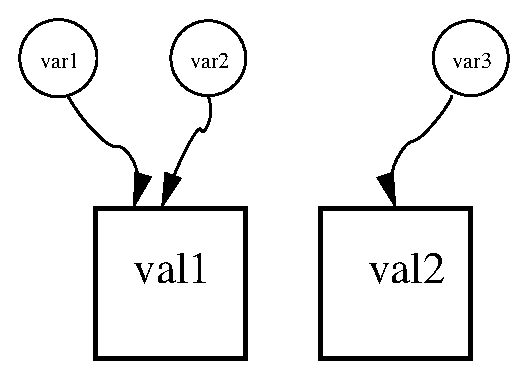
\epsfig{file=figs/share.eps}
\item 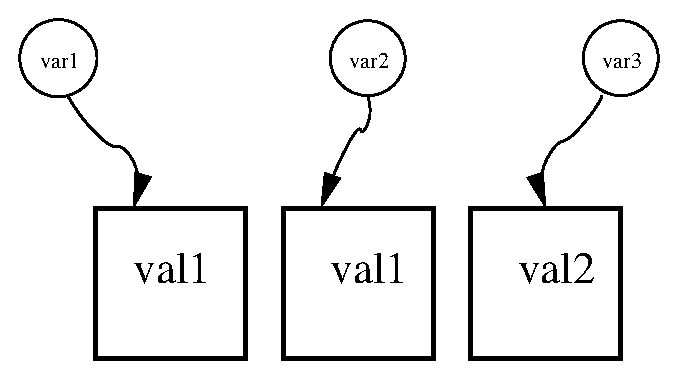
\epsfig{file=figs/fork.eps}
\end{enumerate}
\caption{Before a fork (1), after a fork (2)}
\label{forkfig}
\end{center}
\end{figure}

This subroutine checks whether its input shares its value with
anyone else, and if so, makes a new node of which its input will now
have sole custody (see figure \ref{forkfig}).  
Now the example above can be
modified slightly using \verb+fork+:
\begin{verbatim}
  print *,sum_area(bbox)       ! prints out ``1.0d0''
  abox = bbox 
  call fork(abox)              ! ensure independence of abox
  print *,sum_area(abox)       ! prints out ``1.0d0''
  call normalize(abox)
  print *,sum_area(abox)       ! prints out ``0.0d0''
  print *,sum_area(bbox)       ! prints out ``1.0d0''
\end{verbatim}

The \verb+fork+ constructor, or some similar procedure, allows the
user to establish the independence of \verb+abox+ before modifying it.
In the Java language, where abstract types are (second class) handles,
forking is done by a routine called \verb+clone()+ (e.g. 
\verb+a = b.clone()+).

One appealing alternative syntax to the \verb+fork+ subroutine is
a \verb+box_fork+ constructor (overloading the generic \verb+box+
constructor function), which can be expressed in terms of \verb+fork+
as:
\begin{verbatim}
interface box
  module procedure box_fork
end interface

function box_fork(bx) result(newbx)
  type(box_obj), intent(in) :: bx
  type(box_obj) newbx
  call my(bx,newbx)
  call fork(newbx)
  call bequeath(thy(newbx))
end function box_fork
\end{verbatim}
Its appeal is primarily in the fact that it adds no new procedure names
to the SADR, while giving users the ability fork efficiently.

Handles can be a convenience, but they are counter to
the intuition of the typical FORTRAN programmer.  Additionally, they
can be a serious vulnerability to a software component that needs to
share important, large, pieces of data with other components, yet does
not want to give everyone a license to modify its internal state.
As such, we have not included any handles in the Socorro code.


\subsubsection{Lazy copied values}

\label{lazysec}

Lazy copying is an optimization which prevents excessive copying
that might occur with simple variable size value types, while
still retaining value semantics.  Thus, the user need never
know that he/she is using anything but a first class type.

We define a lazy copied \verb+type(box_obj)+ as a modification of
the handle version of \verb+type(box_obj)+.
With identical implementations of 
\verb+glean+, \verb+bequeath+, \verb+my+, \verb+thy+, and
\verb+assign_box+.  

To create the illusion of regular copying,
the \verb+fork+ subroutine is made private, only callable by functions
in the box module.  The implementer must also identify and modify
every mutator of \verb+type(box_obj)+ to call \verb+fork+ before acting.
\begin{verbatim}
subroutine normalize(bx)    ! a mutating procedure
  type(box_obj), intent(inout) :: bx
  call my(bx)
  call fork(bx)             ! make sure you own the node
  bx%o%area = bx%o%area - sum(bx%o%area)/size(bx%o%area)
  call glean(thy(bx))
end subroutine
\end{verbatim}

The result is a data type that performs like a handle behind the
scenes, copying around lightweight references instead of heavyweight
data.  However, any time a mutator is called, one is assured that it
will happen only on ones own value, since a copy will automatically
occur if the value is shared (this policy is also called
{\em copy on write}).
\begin{verbatim}
  print *,sum_area(bbox)       ! prints out ``1.0d0''
  abox = bbox
  print *,sum_area(abox)       ! prints out ``1.0d0''
  call normalize(abox)
  print *,sum_area(abox)       ! prints out ``0.0d0''
  print *,sum_area(bbox)       ! prints out ``1.0d0''
\end{verbatim}

This type allows for large quantities of data to be shared by
many different components of a program, just as handles do, but
insulates the owner of that data from any tampering from outsiders,
unlike handles.

Lazy copied values are used extensively in the Socorro code to share data
between software components.

\subsubsection{Handles with lazy copied values}

The techniques described so far can be scaled up in a number of ways
implementing a variety of memory management policies.  Here we present
an example that the astute reader might have anticipated.

With one level of indirection, one can diminish the need for excessive
copying, using handles or lazy copied values.  With two levels of
indirection, more sophisticated memory management is possible.  One
structure looks like it might have promise, but which did not find its
way into the current Socorro code is that of handle with a lazy copied
value.  This can be thought of as a handle, that has a lazy
\verb+fork+ command.

This can be achieved by combining the lazy copied type
\verb+type(box_obj)+ described in Section \ref{lazysec}, with the
handle construction of Section \ref{handlesec}.

\begin{verbatim}
type, public:: box_obj    ! a handle with a lazy copied value
private
  integer ref
  type(box_laz), pointer :: o
end type box_obj

type, private:: box_laz    ! a lazy copied value node
private
  integer ref
  type(box_rep), pointer :: o
end type box_laz

type, private:: box_rep   ! defines a value node
private
  integer ref
  integer height,width
  real, pointer :: area(:,:)
end type box_rep
\end{verbatim}

\begin{figure}
\begin{center}
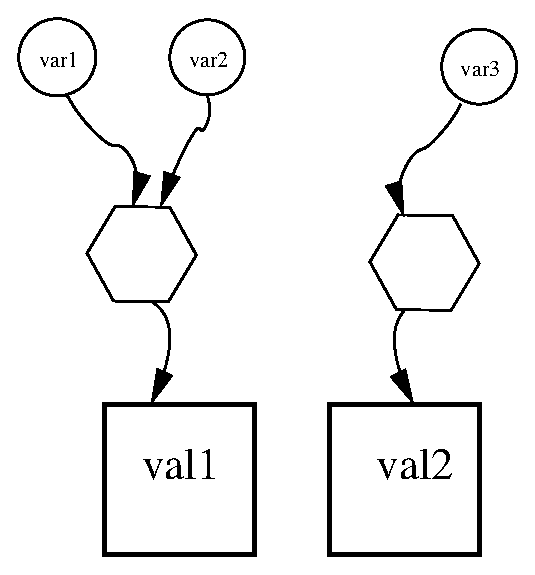
\epsfig{file=figs/complex.eps}
\caption{Additional layer allows for both handle and lazy copying}
\label{complexfig}
\end{center}
\end{figure}

This causes a three-level structure shown in figure \ref{complexfig}
(with the intermediate \verb+type(box_laz)+ represented with
hexagons).  The ref count in \verb+type(box_obj)+ counts the number of
valid identifiers for this variable.  The ref count in
\verb+type(box_laz)+ counts total number of the number of identifiers
using this lazy value.  The ref count in \verb+type(box_rep)+ counts
the number of identifiers using this node value.  In this
implementation.

\begin{verbatim}
subroutine glean(bx)
  type(box_obj) bx
  if (bx%o%o%ref<1) then
    deallocate(bx%o%o%area)  ! get rid of data
    deallocate(bx%o%o)       ! get rid of node
  end if
  if (bx%o%ref<1) then
    deallocate(bx%o)         ! get rid of lazy node
  end if
end subroutine glean

subroutine bequeath(bx)
  type(box_obj) bx
  continue
end subroutine bequeath

interface my
  module procedure my_1arg, my_2arg
end interface my

subroutine my_1arg(bx)
  type(box_obj) bx
  bx%ref = bx%ref+1      ! adopts
  bx%o%ref = bx%o%ref+1  ! number of node users increases too
  bx%o%o%ref = bx%o%o%ref+1
end subroutine my_1arg

subroutine my_2arg(bx_init,bx)
  type(box_obj) bx
  type(box_obj), intent(in) :: bx_init
  bx%o => bx_init%o   ! just swing the pointer
  bx%ref = 1          ! declare initial custody of the box_obj
  bx%o%ref = bx%o%ref+1   ! increase number using the nodes
  bx%o%o%ref = bx%o%o%ref+1
end subroutine my_2arg

function thy(bx) result(bx_out)
  type(box_obj) bx
  type(box_obj) bx_out
  bx%ref = bx%ref -1     ! un-adopt
  bx%o%ref = bx%o%ref -1 
  bx%o%o%ref = bx%o%o%ref -1 
  bx_out%ref = bx%ref    ! create return value
  bx_out%o => bx%o
end function thy

function box(h,w) result(bx)
  integer, intent(in) :: h,w
  type(box_obj) bx
  allocate(bx%o)      ! make a new lazy node
  allocate(bx%o%o)      ! make a new value node
  bx%o%o%height = h
  bx%o%o%width = w
  allocate(bx%o%o%area(h,w))
  bx%o%o%area = 0.0
  bx%ref = 0       ! make orphan
  bx%o%ref = 0
  bx%o%o%ref = 0
end function box

subroutine assign_box(bx,bx_in)
  type(box_obj),intent(inout) :: bx
  type(box_obj),intent(in) :: bx_in
  type(box_obj) bx_tmp
  bx_tmp%o => bx%o    ! may need to glean up the old value
  bx%o%ref = bx%o%ref - bx%ref  ! swing pointer and move ref's
  bx%o%o%ref = bx%o%ref - bx%o%ref
  bx%o => bx_in%o
  bx%o%ref = bx%o%ref + bx%ref
  bx%o%o%ref = bx%o%o%ref + bx%ref
  call glean(bx_tmp) 
  call glean(bx_in)
end subroutine assign_box

subroutine fork(bx)              ! for copying lazy nodes
  type(box_obj) bx
  type(box_laz), pointer :: node
  if (bx%o%ref>bx%ref) then      ! if bx doesn't own lazy node
    allocate(node)               ! make a new lazy node
    node%ref = 0
    node%o => bx%o%o             ! point lazy node to value node
    bx%o%ref = bx%o%ref - bx%ref    ! swing pointers
    bx%o => node
    bx%o%ref = bx%o%ref + bx%ref    ! don't need to change %o%o%ref's
  end if
  glean(bx)
end subroutine fork

subroutine, private :: val_fork(bx) ! the lazy node fork
  type(box_obj) bx
  type(box_rep), pointer :: node
  if (bx%o%o%ref>bx%o%ref) then  ! if lazy node doesn't own value
    allocate(node)               ! make a new value
    node%ref = 0
    allocate(node%area(bx%o%o%height,bx%o%o%width))
    node%area = bx%o%o%area       ! copy allocated stuff
    node%height = bx%o%o%height   ! copy unallocated stuff
    node%width = bx%o%o%width
    bx%o%o%ref = bx%o%o%ref - bx%o%ref    ! swing lazy node's pointers
    bx%o%o => node
    bx%o%o%ref = bx%o%o%ref + bx%o%ref
  end if
  glean(bx)
end subroutine val_fork

\end{verbatim}

One notices two forks, a public one which forks the obj/laz connection
and a private one which forks the laz/rep connection (see figures
\ref{complexforkfig} and \ref{complexfork2fig}).

\begin{figure}
\begin{center}
\epsfig{file=figs/complexfork.eps}
\caption{Forking a handle simply creates a new lazy-copied value}
\label{complexforkfig}
\end{center}
\end{figure}

\begin{figure}
\begin{center}
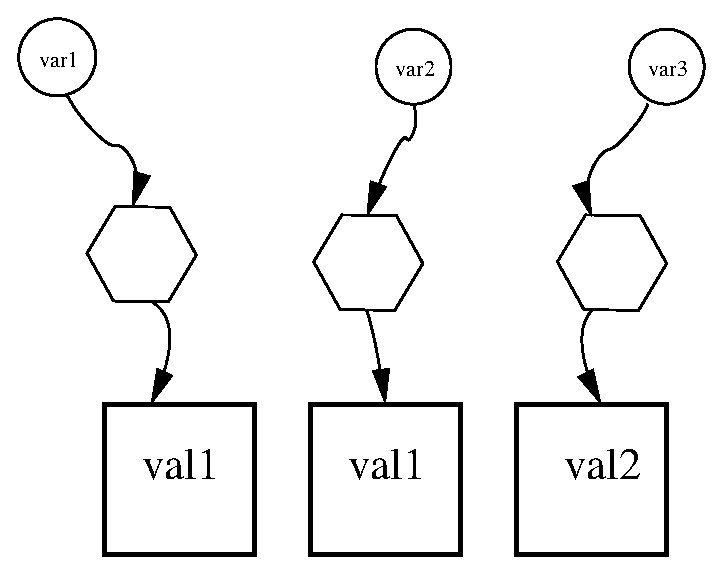
\epsfig{file=figs/complexfork2.eps}
\caption{Mutating a handle forks the node value}
\label{complexfork2fig}
\end{center}
\end{figure}

When the user calls \verb+fork+, a new lazy node is spawned, but no
large copying takes place.  Meanwhile, the implementer of the box abstraction
must use \verb+val_fork+ in order to give the illusion of lazy copying.

In the \verb+normalize+ example:
\begin{verbatim}
subroutine normalize(bx)    ! a mutating procedure
  type(box_obj), intent(inout) :: bx
  call my(bx)
  call val_fork(bx)          ! make sure lazy node owns the value
  bx%o%o%area = bx%o%o%area - sum(bx%o%o%area)/size(bx%o%o%area)
  call glean(thy(bx))
end subroutine
\end{verbatim}

The user does not see a difference between using this type and the
handle type.
\begin{verbatim}
  print *,sum_area(bbox)       ! prints out ``1.0d0''
  abox = bbox; call fork(abox)
  cbox = bbox; call fork(cbox) ! abox,bbox,cbox now have the same 
                               ! value node and differing lazy nodes
  print *,sum_area(abox)       ! prints out ``1.0d0''
  call normalize(abox)         ! value node copy for abox
                               ! bbox, cbox still have same value nodes
  print *,sum_area(abox)       ! prints out ``0.0d0''
  print *,sum_area(bbox)       ! prints out ``1.0d0''
  print *,sum_area(cbox)       ! prints out ``1.0d0''
  call normalize(cbox)         ! value node copy for cbox
  print *,sum_area(bbox)       ! prints out ``1.0d0''
  print *,sum_area(cbox)       ! prints out ``0.0d0''
\end{verbatim}
However, from a performance standpoint, only one substantial copy
occurs at the point where \verb+abox+ or \verb+cbox+ are mutated.
Where the regular handle implementation decreases copying by
sharing values, the only way to protect the data in one handle from
being mutated by actions on another handle is to call \verb+fork+
which is implemented by copying.  In this implementation, the
call to \verb+fork+ is implemented via lazy copying, so the data
is protected, without necessarily incurring substantial copying
expense until an attempt is made to mutate the \verb+fork+-ed handle.

Handles with lazy copied values, would seem to be an ideal way for
software components to both protect their data and allow portions
of their data to be modified by outside components.  Like handles,
however, they do not behave like first class types, and would
therefore be counter-intuitive to FORTRAN programmers, so we have
yet to implement them in Socorro.

We should also comment that in languages with support for indirection
and overloaded indirection, like C++ or Perl, one could implement
a handle with lazy copied values as a simple extension of a lazy copied value
type, having both the lazy type and the handles to the lazy type 
coexisting and sharing code.  This is not so easy in FORTRAN unfortunately.

\subsection{Memory management and scaling}

One important point left to be discussed about the SADR rules is how
they scale in a data hierarchy.  The design of the interface went
through a couple iterations, for it was found that some versions,
which worked fine for types with intrinsic members, could not easily
be applied to higher level types with their own garbage collected members.

A prototypical higher-order (lazy copied) type could be defined as follows:
\begin{verbatim}
    type, public :: high_obj
    private
      integer ref
      type(high_rep), pointer :: o
    end type

    type, public :: high_rep
    private
      integer  ref
      type(low_obj)  :: mem   ! note member is a SADR type
      real*8 other
    end type

    subroutine glean(h)
      type(high_obj) h
      if (h%o%ref<0) then
        call glean(h%mem)
        deallocate(h%o)
      end if
    end subroutine

    subroutine bequeath(h)
      type(high_obj) h
      continue
    end subroutine

    subroutine my_1arg(h)
      type(high_obj) h
      h%ref = h%ref +1
      h%o%ref = h%o%ref +1
    end subroutine

    subroutine my_2arg(hin,hout)
      type(high_obj) hin,hout
      hout%ref = 1
      hout%o => hin%o
      hout%o%ref = hout%o%ref +1
    end subroutine

    function thy(h) result(hout)
      type(high_obj) h,hout
      h%ref = h%ref -1
      h%o%ref = h%o%ref -1
      hout%ref = h%ref
      hout%o => h%o%ref
    end function

    function high(l,ot) result(h)
      type(high_obj) h
      type(low_obj), intent(in) ::l
      real*8, intent(in) :: ot
      h%ref = 0
      allocate(h%o)
      h%o%ref = 0
      call my(l,l%o%mem)
      h%o%other = ot**2
    end
\end{verbatim}

We see that it is only necessary to \verb+my+ the \verb+%mem+
member of \verb+type(high_obj)+ once upon creation and to \verb+thy+
it just once when \verb+type(high_obj)+ is being deconstructed by
\verb+glean+.  Another way to say this is membership in another value
counts as one reference.  In doing so, we avoid the need to traverse
all the data members of the higher type recursively (for a complicated
data structure this would be unnecessarily expensive).

The reader will also notice that because constructors are
functions, one need not declare intermediate results just to
initialize a higher-order data type.  The initialization of
\verb+h+ of type \verb+type(high_obj)+,
\begin{verbatim}
      type(low_obj)  tmp
      ....
      call my(low(1,2,3), tmp)   ! initialize a temporary
      call my(high(tmp,9),  h)   ! initialize h
      call glean(thy(tmp))       ! get rid of temp
      ....
\end{verbatim}
can be optimized to
\begin{verbatim}
      ....
      call my(high(low(1,2,3),9.0d0),h)
      ....
\end{verbatim}
saving three unnecessary lines of program text as well as being
more memory efficient if real copies are done in the initialization.
If \verb+type(low_obj)+ also has a SADR member, there would be
three more unnecessary lines in the first pattern.
In fact, the first construction pattern has three unnecessary lines of 
text for every SADR type which requires initialization, that
would add about fifteen unnecessary lines to the initialization
of Socorro's \verb+type(config_obj)+.  For this reason,
we caution anyone serious
about creating hierarchical data not to adopt the sort of
\verb+call new()+ and \verb+call delete()+ syntax which has been
suggested in \cite{KimLeeMartin.OORI,DecykNotronSzymanski.OOF90}

Finally, we present an example of a fork routine which minimizes
copying in a hierarchy.  Let's us suppose that \verb+type(high_obj)+
and \verb+type(low_obj)+ are to be lazy copied values.  The fork
would be
\begin{verbatim}
subroutine fork(h)              ! for coping handles
  type(high_obj) h
  type(high_rep), pointer :: node
  if (h%o%ref>h%ref) then      ! if h doesn't own the node
    allocate(node)               ! make a new node
    node%ref = 0
    call my(h%o%mem,node%mem)    ! (lazy) copy value
    node%other = h%o%other       ! copy value
    h%o%ref = h%o%ref - h%ref    ! swing pointers
    h%o => node
    h%o%ref = h%o%ref + h%ref
  end if
  glean(h)
end subroutine fork
\end{verbatim}
where one notes that there is not nor needs to be any recursive call
to low's \verb+fork()+ procedure (which should be private anyhow).
Since only lazy copying is performed on the members, no 
lazy copied member is
really copied on the fork until that member is modified (see figure
\ref{lch}).

\begin{figure}
\begin{center}
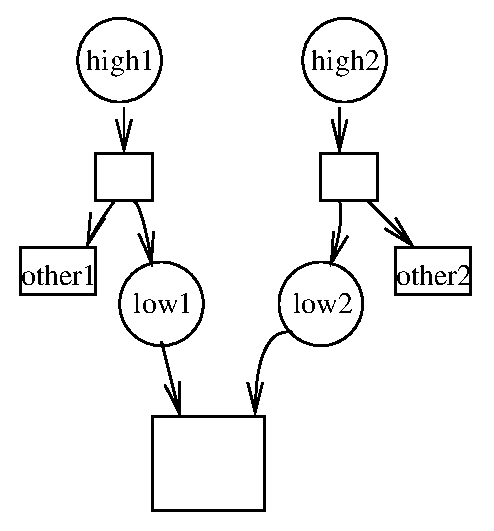
\epsfig{file=figs/lc_hierarchy.eps}
\caption{Example of lazy copying in a hierarchy}
\label{lch}
\end{center}
\end{figure}

In complicated hierarchies, this allows copying to be avoided
separately for each member of the complex (see figure \ref{biglch}).
\begin{figure}
\begin{center}
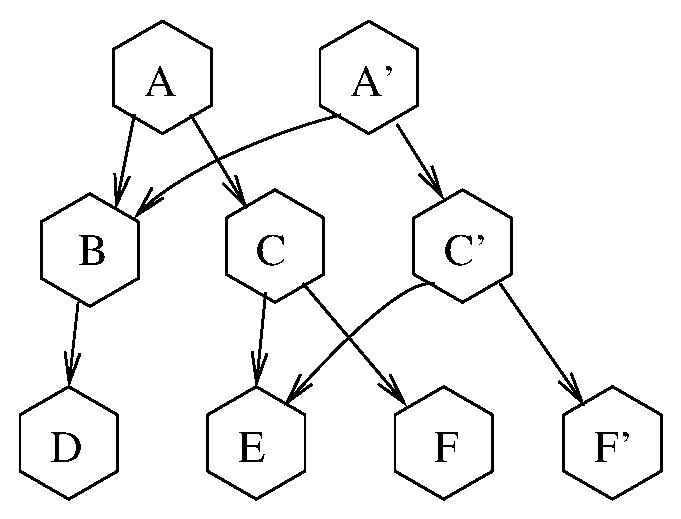
\epsfig{file=figs/biglc_hierarchy.eps}
\caption{Example of lazy copying in a complicated hierarchy (condensing
different abstract types into hexes).  This results from copying 
A and modifying F.}
\label{biglch}
\end{center}
\end{figure}
This keeps real copying to a minimum.


\section{Socorro Modular structure}

What follows will be a description of the current Socorro code
structure as well as a description of more specific tricks and
techniques we have employed in the code.  Let the reader be warned
that the Socorro code is in a perpetual state of development, and
that this section is meant to give enough of a framework
to the reader so that he/she can look over any module in Socorro
with some idea as to its purpose.

While the debate rages on between the use of global versus local
variables in the FORTRAN community, Socorro encapsulates almost all
program state into a single variable of \verb+type(config_obj)+ (the
various runtime support functions are the only exception to this).
The initialization of a variable of \verb+type(config_obj)+
is the entire self-consistent calculation.

The \verb+type(config_obj)+, its constituent types and the rest of
their descendants can be rendered in a graph shown in figure
\ref{datafig}.  Each module in the diagram is responsible for
maintaining its own rep-invariants.  If the \verb+config_mod+
module defines a function which modifies the \verb+type(external_obj)+
of variable of \verb+type(config_obj)+, that function must also
restore the self-consistency of the \verb+type(config_obj)+ variable
as that is one of the rep-invariant of \verb+type(config_obj)+.

The universal application of this principle drives all computation
in Socorro, currently.  All mutable types in Socorro
come with an \verb+update()+ subroutine, which allows them to
modify their constituents and perform whatever necessary computations
must be done to restore the rep-invariants (see figure \ref{modifyfig}).
One technique we are using to implement this efficiently is
discussed in section \ref{ghostsec}.

\begin{figure}
\begin{center}
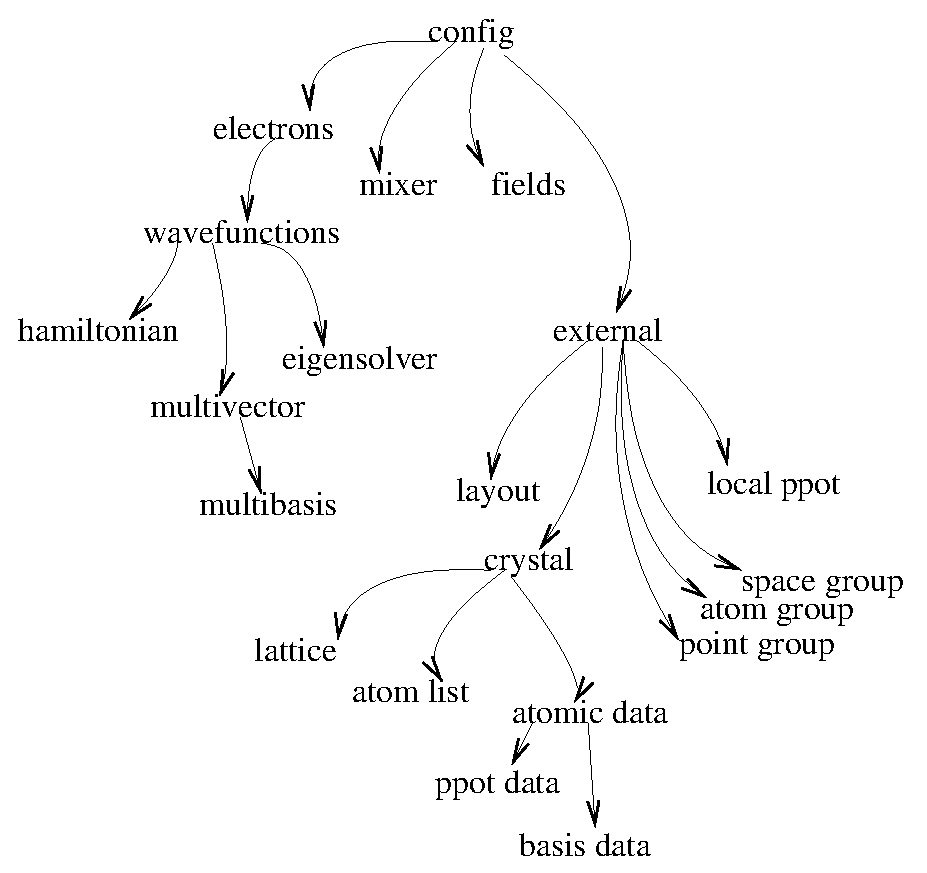
\epsfig{file=figs/datamap.eps}
\caption{A map of the data hierarchy in Socorro}
\label{datafig}
\end{center}
\end{figure}

\begin{figure}
\begin{center}
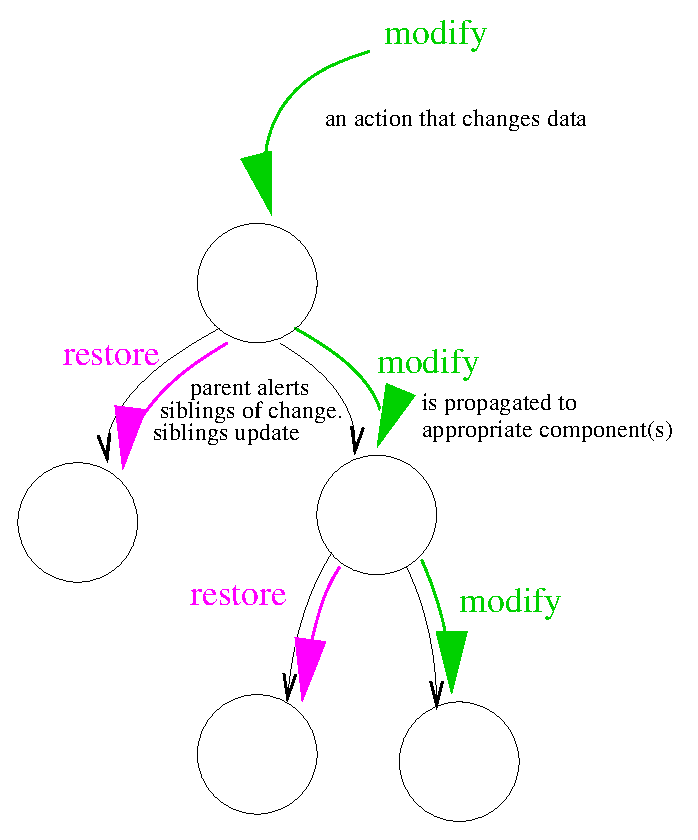
\epsfig{file=figs/constraint.eps}
\caption{Iterative dynamics are driven by the preservation of representation
invariants.}
\label{modifyfig}
\end{center}
\end{figure}

\subsection{Documentation}

People who program do not like to document what they write.
This is a sociological fact.  The person who writes a program,
when he/she does document, will tend to forgive the brevity
or opaqueness of his commentary.  This is a psychological fact.
In light of these two facts, it is best to adopt a documentation
process which minimizes effort in both creation and modification
of program documentation.

The free form Socorro files place procedure comments in the
procedure headers and allow the implementer the option of exporting
arbitrary code into the documentation for that module, to spare
him/her the tiresome task of recasting the same information into
the documentation.  Exporting code to documentation
prevents the documentation and code
from drifting apart.  Note: the fixed form Socorro files (which
will eventually be converted to free form) follow
an earlier convention which was abandoned primarily because
it promoted code/doc drift.

Documented blocks of code start with a line which begins with the
string \verb+!doc$+ in the program text.  If anything else is on that
line, it is stripped of the \verb+!doc$+, capitalized, and exported.
All subsequent lines are exported (stripping out leading \verb+!+
symbols), until the next occurrence of a \verb+!cod$+ which terminates
the documentation block.

For example, the following module header,
\begin{verbatim}
!doc$
      MODULE LATTICE_MOD

!     The lattice module hold basic lattice concepts: the lattice vectors
!     the lattice reciprocal vectors.

      use kind_mod
      use core_mod
      use diary_mod
      use arg_mod
      use math_mod
      use ghost_mod

!cod$

      real (wpd), parameter :: tol_nbhd = 1.0d-8

      type lattice_obj
      private
      type(ghost) :: g
      real(wpd) :: lconstant
      real(wpd), dimension(3,3) :: vectors
      real(wpd), dimension(3,3) :: ivectors
      end type
!doc$ 
!     defines a type(lattice_obj)

!cod$     
\end{verbatim}
has the following documentation 
\begin{verbatim}
      MODULE LATTICE_MOD

      The lattice module hold basic lattice concepts: the lattice vectors
      the lattice reciprocal vectors.

      use kind_mod
      use core_mod
      use diary_mod
      use arg_mod
      use math_mod
      use ghost_mod


      defines a type(lattice_obj)

\end{verbatim}

All Socorro modules export their \verb+use+ information to help check
for dependencies, a \verb+public+ declaration block which lists all
public functions defined therein, as well as a specification for each
publicly declared function using the clauses listed in section
\ref{specsec}.  The specification for a function is intimately
intertwined with the actual function header:

\begin{verbatim}
      function cons_load(prefix) result(lat)
!doc$ function lattice(prefix) result(lat)
      type(lattice_obj) lat
      character(*), intent(in) :: prefix
!     requires : existence of the file (see effects), non-sigularity of
!                the vectors in the file
!     effects  : like previous constructor only reads latc and vector
!                information from file prefix//"lat"
!     errors   : format problems or IO problems

!cod$
\end{verbatim}
which translates to
\begin{verbatim}
      function lattice(prefix) result(lat)
      type(lattice_obj) lat
      character(*), intent(in) :: prefix
      requires : existence of the file (see effects), non-singularity of
                 the vectors in the file
      effects  : like previous constructor only reads latc and vector
                 information from file prefix//"lat"
      errors   : format problems or IO problems
\end{verbatim}

In practice, the programmer overhead is minimal.  There is negligible
effort to exporting public names and argument types, and little more
effort to write a few specification clauses.  Module maintainers can
view the specification of each procedure on the same page as the
implementation they are maintaining.  This encourages better auditing
to ensure consistency with the specification, as well as allowing
others to more easily critique and improve upon the specification.

Primary documentation is generated by running one of two scripts (one
for free form and one for fixed) which pull out the documentation
blocks for each file and writes them to a corresponding file.  In
this form, the documentation can be transformed to a secondary form like HTML
for some sort of cross-referencing links.

\subsection{Error handling}

\label{errorsec}

An error is, at worst, a program crash, and, at best, an abnormal exit from
a procedure (because a condition was checked which anticipated a program
crash).  Assuming that an error is detected and an abnormal exit occurs,
the caller of the erring procedure must be prepared to respond to the exit.
There are, roughly, three levels of error response: 

\begin{itemize}
\item Catch the error, recover appropriately, an proceed as normal after.
\item Catch the error and fair to recover, and exit abnormally.  This is
called {\em error propagation}.
\item Check nothing and proceed normally with whatever partial results 
the procedure  has returned.  Some languages have runtime exception handling
which forces the caller to at least propagate all uncaught exceptions (e.g.
Java ,C++).
\end{itemize}

FORTRAN does not support runtime exception handling.  This makes a
general framework for error recovery impossible.  However, it is
possible to detect and propagate errors by a programmer convention.
One of Socorro's support modules, \verb+core_mod+, defines a private
module logical variable which, is initially false, can be checked, and
can set to true when an error is detected.  It provides two public error
functions which allow the user to check for a potential error condition
and to propagate errors.

Programmers are optimists.  That is why they need debuggers.  When a set
of complicated functions with various error conditions are strung
together, it is assumed that they will work without error.  Although
this optimism will probably never be cured, we can attempt to make is
as easy as possible for the programmer to participate in the error
handling conventions.  We have designed the error specification so 
that error propagation takes only one line of code (it seemed unlikely
that programmers would want to devote more lines to the error handling
than the call itself).  Error propagation typically is
\begin{verbatim}
    call this_could_err(1,2,3)
    ! check to propagate error
    if (error('an error happened here')) goto exit_label:
\end{verbatim}
which checks to see if the program is in a state of error after the
call to \verb+this_could_err+.  If not, false is returned and the
branch is not executed.  If so, the string argument, which helps trace
the error, is written to the error output file(s), true is returned
and the branch is taken, resulting in the abnormal exit.  There is
also a one-line call which checks for an error and then exits: 
\begin{verbatim}
    ! check to generate error
    if (error(k > n, 'K should be <= N')) goto exit_label:
\end{verbatim}
Here if the first argument is false, and the program is not currently in
a state of error, false is returned and the branch is not taken.  If
the first argument is true or the program is already in a state of error,
the second argument is written to the error output, true is returned, and
the branch is taken.

More specific documentation of the error services is found in the
\verb+core_mod+ module.

\subsection{Parallelism}

Socorro is designed to run in a parallel environment.  This is an
atypical feature of most parallel codes, which are ``parallelized''
serial codes.  It is our opinion that parallelization as an
afterthought causes what might have been a good design to lose a lot
of its integrity.  The first Socorro module that was ever written was
the \verb+core_mod+ module which supplies primitives for file I/O,
communication, and error handling.

The communication primitives are essentially wrappers for MPI calls,
implementing basic MPI procedures and presenting the user with a
simplified interface to MPI.  These wrappers are used by every other
procedure in Socorro.  Thus, should the parallel interface change, or
should a serial version be desired, this would require re-implementing
the core module and only minor modifications to the rest of Socorro.

The file I/O system is a set of logical functions which one employs
upon data of type \verb+type(file_obj)+ to preface the usual read and
write statements.

\begin{verbatim}
      type(file_obj), public :: f
      call my(file(name),f)
      if (i_access(f)) open(x_unit(f),x_name(f))
      if (i_access(f)) read(x_unit(f),*) data; if (i_comm(f)) scatter_commands
      if (i_access(f)) call close(x_unit(f))
      if (i_access(f)) open(x_unit(f),x_name(f))
      if (i_comm(f)) gather_commands; if (i_access(f)) write(x_unit(f),*) data
      if (i_access(f)) call close(x_unit(f))
      call glean(thy(f))
\end{verbatim}     

The advantage of having these primitives centrally located is that it
allows the tailor of the file access behavior to the form of file
access of the programming environment (e.g. only the root process has
file access, separate file systems for each process, etc).

The error system was described in section \ref{errorsec}.

\subsection{Ghosts}

\label{ghostsec}

In order for data components in the hierarchy to check their
consistency with each other efficiently, it is important that
components be able to cheaply tell when another component has changed
from when it was last used.

For example, if one modifies a copy of the \verb+type(crystal_obj)+
component (called \verb+cr+) of a variable of
\verb+type(external_obj)+ (called \verb+ext+), by changing 
its \verb+type(atoms_obj)+ component, then when the
\verb+update(ext,cr)+ call is made, it would be more efficient if
\verb+ext+ could figure out that only the lattice changed, and thus
modifying those components which depend on that information (its
\verb+type(local_ppot)+ and \verb+type(space_group)+) while not having to 
update its other components (the two \verb+type(point_group)+'s, the
\verb+type(layout_obj)+).  The \verb+update+ routine can decide this
based on a comparison of the new crystal's components 
against the old crystal's components.

To do this cheaply, we decided that to put unique identifiers in most
of the Socorro data types.  The identifiers are called {\em ghosts},
are of a fixed size auxiliary \verb+type(ghost)+ which are defined
by the short module specified by:

\begin{verbatim}
      module GHOST_MOD

      This module defines the unique identifier system that
      is used to determine identity among various components in
      Socorro.

      public :: operator(.eq.), operator(.ne.), x_ghost

      FUNCTION X_GHOST() RESULT(G)
      type(ghost) :: g
      effects: returns a new unique ghost

      OPERATOR(.EQ.)(G1,G2)
      type(ghost), intent(in) :: g1, g2
      effects: tests ghosts g1 and g2 for equality

      OPERATOR(.NE.)(G1,G2)
      type(ghost), intent(in) :: g1, g2
      effects: tests ghosts g1 and g2 for inequality

\end{verbatim}

Thus, when a new value is created or modified, it can be assigned a
unique identifier.  This identifier can compared with the identifiers
of other data.  Most importantly, however, the ghost of component
\verb+A+ can be cached by component \verb+B+ and used by
\verb+B+ to detect changes in component \verb+A+.

Here is an example of how ghosts relate to update functions taken from the
\verb+update+ function in module \verb+multibasis_mod+.
\begin{verbatim}
       subroutine update_wb_crys(wb,crys)
!doc$ subroutine update(wb,crys)
        type(multibasis_obj) , intent(inout) ::wb
        type(crystal_obj), intent(in) :: crys
!     effects: modifies wb with respect to a change in the crystal. wb will
!       assume the same layout and the same mapping from grid points to
!       basis points (e.g. the dimension of the multibasis never changes).  
!       If one wishes to maintain consistency between the proto-basis and 
!       the crystal, one should use multibasis()

!cod$
        real(double), dimension(3) :: fkpt,v,w
        call my(wb)
        call my(crys)
!!!!!!!!! check lattice's ghost against cached lattice ghost to see if
!!!!!!!!! the update can be safely skipped.
        if (x_ghost(x_lattice(crys)).ne.x_ghost(wb%o%lat)) then
!!!!!!!!!!!! do the update
           call own(wb)
           wb%o%ghost = x_ghost()
           wb%o%fkpt = lat2f(x_lattice(crys),f2lat(wb%o%lat,wb%o%fkpt))
           ng = size(wb%o%gpt,2)
           do ig = 1,ng
              v = (/wb%o%gpt(1,ig),wb%o%gpt(2,ig),wb%o%gpt(3,ig)/)
              w = lat2f(x_lattice(crys),f2lat(wb%o%lat,v))
              wb%o%gpt(1,ig) = w(1)
              wb%o%gpt(2,ig) = w(2)
              wb%o%gpt(3,ig) = w(3)
           end do
           wb%o%lat = x_lattice(crys)
           wb%o%cellvol = x_unitcv(wb%o%lat)
        end if
100     if (error("update_wb_crys: ")) continue
        call glean(thy(wb))
        call glean(thy(crys))
      end subroutine update_wb_crys
\end{verbatim}
Since a variable of \verb+type(multibasis_obj)+ must stay
up to date with some \verb+type(lattice_obj)+, it must react
when that variable changes.  The ghost check allows for 
some unnecessary computation to be avoided.

This is really nothing more than the old trick of using three integer
\verb+SAVE+ variables in some FFT wrappers to cache the dimensions of the
input data so that the wrapper would only automatically generate new
FFT-plans when the dimensions of the input data changed.  We have
simply generalized it so that the identities of abstract types can be
cached just as easily.


\subsection{Grid example}

As a final tutorial introduction to the Socorro code, we will
do a full explication of one very much used Socorro type, the
\verb+type(grid_obj)+.  Variables of \verb+type(grid_obj)+ are
designed to represent parallel and serial data in Fourier
and position space in a way that allows interconversions to be
called behind the scenes.  \verb+type(grid_obj)+ is used extensively
by routines that work with the various fields as a means of packaging
and unpackaging arguments and results.


\begin{figure}
\begin{center}
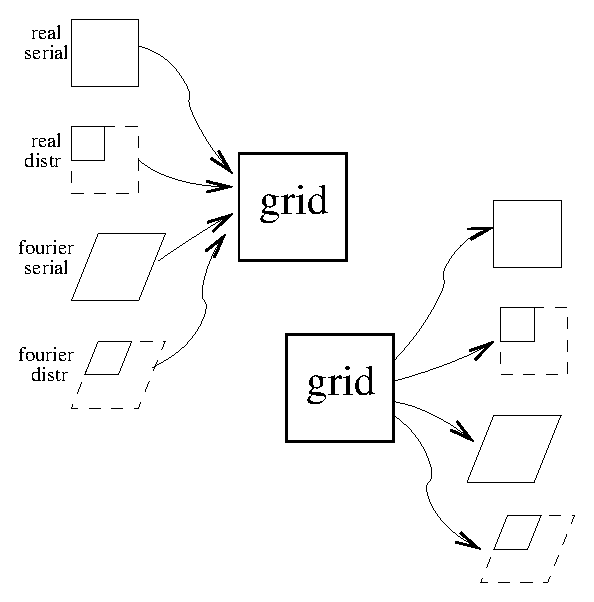
\epsfig{file=figs/grid.eps}
\caption{The grid type is used to glue together various field formats
as a general union operator}
\label{gridfig}
\end{center}
\end{figure}

The point of this section is to walk the reader through one Socorro
module and explain the general look and feel, so the reader can more
easily absorb the more complicated data types.  We use the source
\verb+grid_mod.f90+ from the date {Sep 26 16:03:21 MDT 2000},
with comments in the program text mostly stripped out, and lines
wrapped.

\begin{verbatim}
      module grid_mod

      use kind_mod
      use ghost_mod
      use core_mod
      use layout_mod

      private
\end{verbatim}
The grid module depends on only a few other modules.  Most notable of
these is the \verb+layout_mod+ which contains the primitive redistribution
and transformation functions that will be called from this module.  We
set the module private by default as in all Socorro modules to avoid
accidentally making internal functions public.

\begin{verbatim}
      type, public :: grid_obj
      private
      integer :: ref
      type(grid_ref), pointer :: o
      end type

      type grid_ref
      integer :: ref
      type(ghost) :: g
      integer :: type
      type(layout_obj) :: layout
      real(wpd), dimension(:,:,:), pointer :: rdata
      complex(wpd), dimension(:,:,:), pointer :: cdata
      end type 
\end{verbatim}
The internals of grid consist of a ghost field, a type field, a copy
of the layout to use in redistribution, and two data pointers.  The 
rep-invariant can be summarized by the following list of allowed states:
\begin{itemize}
\item type is \verb+EMPTY_KIND+: cdata is null, rdata is null
\item type is \verb+RS_KIND+   : cdata is null, rdata is serially dimensioned
\item type is \verb+RD_KIND+   : cdata is null, rdata is distributedly dimensioned
\item type is \verb+CSP_KIND+  : rdata is null, cdata is serially dimensioned
\item type is \verb+CDP_KIND+  : rdata is null, cdata is distributedly dimensioned
\item type is \verb+CSF_KIND+  : rdata is null, cdata is serially dimensioned
\item type is \verb+CDF_KIND+  : rdata is null, cdata is distributedly dimensioned
\end{itemize}
where ``dimensionalization is determined by the layout'' is equivalent to
the logical function \verb+consistent(\{rc\}data,layout,type)+ defined in
the module \verb+layout_mod+.

What then follows are the declarations of a whole bunch of 
overloaded functions.  The \verb+public+ declarations at the bottom
of this section summarize the public interface.
\begin{verbatim}
      interface grid
      module procedure grid_const
      end interface
      interface my
      module procedure my_grid, my_grid_new
      end interface
      interface thy
      module procedure thy_grid
      end interface
      interface bequeath
      module procedure bequeath_grid
      end interface
      interface glean
      module procedure glean_grid
      end interface
      interface take
      module procedure take_ptr_grid_r,take_ptr_grid_c
      end interface
      interface put
      module procedure put_ptr_grid_r,put_ptr_grid_c
      end interface
      interface x_type
      module procedure grid_type
      end interface
      interface x_layout
      module procedure grid_layout
      end interface
      interface x_ghost
      module procedure grid_ghost
      end interface
      interface assignment(=)
      module procedure assign_grid
      end interface

      public :: grid,my,thy,glean,bequeath,assignment(=)
      public :: x_type, x_layout, put, take
      public :: x_ghost
\end{verbatim}
Aside from the SADR functions, and functions to extract different
members of \verb+type(grid_obj)+, there are really two major functions
defined \verb+put+ which puts data on the grid and \verb+take+ which
takes data off the grid.

The garbage collection is just the simple lazy copied value method defined
in section \ref{lazysec}.  (Note: some of the private names for the overloaded
SADR procedures might vary from the examples in \ref{lazysec}.)

\begin{verbatim}
      subroutine my_grid_new(gi,G)
      type(grid_obj) ::gi,g
      g%ref = 1
      g%o => gi%o
      g%o%ref = g%o%ref+1
      end subroutine

      subroutine my_grid(G)
      type(grid_obj) g
      g%ref = g%ref+1
      g%o%ref = g%o%ref+1
      end subroutine

      function thy_grid(G) result(gout)
      type(grid_obj)::g,gout
      g%ref = g%ref-1
      g%o%ref = g%o%ref-1
      gout%ref = g%ref
      gout%o => g%o
      end function

      subroutine bequeath_grid(G)
      type(grid_obj) g
      continue
      end subroutine

      subroutine glean_grid(G)
      type(grid_obj) g
      if (g%o%ref<1) then
         select case (g%o%type)
         case (EMPTY_KIND)
            continue
         case (RD_KIND,RS_KIND)
            deallocate(g%o%rdata)
         case (CSP_KIND,CDP_KIND,CSF_KIND,CDF_KIND)
            deallocate(g%o%cdata)
         end select
         deallocate(g%o)
      end if
      end subroutine

      subroutine assign_grid(g1,g2)
      type(grid_obj), intent(inout) :: g1
      type(grid_obj), intent(in) :: g2
      type(grid_obj) gtmp
      call my(g2)
      if (error(x_ghost(g1%o%layout).ne.x_ghost(g2%o%layout), &
          "assigning grids of unequal layouts")) goto 100
      gtmp%o => g1%o
      g1%o%ref = g1%o%ref - g1%ref
      g1%o => g2%o
      g1%o%ref = g1%o%ref + g1%ref
      call glean(gtmp)
 100  call glean(thy(g2))
      end subroutine

\end{verbatim}

The grid constructor is defined by
\begin{verbatim}
      function grid_const(ly) result(g)
      type(grid_obj) g
      type(layout_obj), intent(in) :: ly
      g%ref = 0
      allocate(g%o)
      g%o%g = x_ghost()
      g%o%ref = 0
      g%o%type = EMPTY_KIND
      call my(ly,g%o%layout)
      nullify(g%o%rdata)
      nullify(g%o%cdata)
      end function
\end{verbatim}
which returns an empty grid to the caller.

\begin{verbatim}
      integer function grid_type(g)
      type(grid_obj), intent(in) :: g
      call my(g)
      grid_type = g%o%type
      call glean(thy(g))
      end function

      type(layout_obj) function grid_layout(g)
      type(grid_obj), intent(in) :: g
      call my(g)
      call my(g%o%layout,grid_layout)
      call bequeath(thy(grid_layout))
      call glean(thy(g))
      end function

      type(ghost) function grid_ghost(g)
      type(grid_obj), intent(in) :: g
      call my(g)
      grid_ghost = g%o%g
      call glean(thy(g))
      end function
\end{verbatim}
The functions above allow relevant information to be extracted
from grids like ghosts, the type of the currently stored
grid data, as well as the underlying layout of the grid itself
if needed.  All these functions have the property that they 
are cheap to call and do not have any side effects.
We got it into our heads to put an \verb+x_+ prefix in front of
such functions, and the convention generally stuck.

We can now move to those functions which mutate grid data.

\begin{verbatim}
      subroutine mutate_i(g)
      type(grid_obj) g
      type(grid_obj) gtmp
      if (g%ref < g%o%ref) then
         allocate(gtmp%o)
         gtmp%o%ref = 0
         call my(g%o%layout,gtmp%o%layout)
         gtmp%o%type = g%o%type
         select case (g%o%type)
         case (EMPTY_KIND)
            continue
         case (RD_KIND,RS_KIND)
            call alloc(gtmp%o%rdata,g%o%layout,g%o%type)
            gtmp%o%rdata = g%o%rdata
            nullify(gtmp%o%cdata)
         case (CSP_KIND,CDP_KIND,CSF_KIND,CDF_KIND)
            call alloc(gtmp%o%cdata,g%o%layout,g%o%type)
            gtmp%o%cdata = g%o%cdata
            nullify(gtmp%o%rdata)
         end select
         gtmp%o%g = g%o%g
         g%o%ref = g%o%ref - g%ref
         g%o => gtmp%o
         g%o%ref = g%o%ref + g%ref
      end if
      end subroutine
\end{verbatim}
In \verb+grid_mod+ the function for forking off a new grid is 
the private function \verb+mutate_i+.

\begin{verbatim}
      subroutine empty_grid_i(G)
      type(grid_obj), intent(inout) :: g
      select case (g%o%type)
      case (EMPTY_KIND)
         continue
      case (RD_KIND,RS_KIND)
         deallocate(g%o%rdata); nullify(g%o%rdata)
      case (CSP_KIND,CDP_KIND,CSF_KIND,CDF_KIND)
         deallocate(g%o%cdata); nullify(g%o%cdata)
      end select
      g%o%type = EMPTY_KIND
      end subroutine
\end{verbatim}
This is an internal utility to make sure a grid has no data on
it when new data is about to be put on it.  One notes that it
does not call \verb+mutate_i+ even though it modifies its argument,
but since it is a private procedure and is never called in a
context where forking is needed, that is ok.

\begin{verbatim}
      subroutine put_ptr_grid_r(DATA,G,kind)
      real(wpd), dimension(:,:,:), pointer :: data
      type(grid_obj), intent(inout) :: g
      integer, intent(in)    :: kind
      integer tpo
      real(wpd), dimension(:,:,:), pointer :: rtmp
      complex(wpd), dimension(:,:,:), pointer :: ctmp
      tpo = kind
      call my(g)
      call mutate_i(g)
      call empty_grid_i(g)
      if (error(.not.consistent(data,g%o%layout,kind), &
           "put_ptr_grid_r: inconsistent type for data")) goto 100
      rtmp => data;  nullify(ctmp);  nullify(data)
      call transfer_grid(g%o%layout,G%o%TYPE,G%o%RDATA,G%o%CDATA,  &
                         TPO,RTMP,CTMP)
      g%o%g = x_ghost()
 100  if (error("put_ptr_grid_r: ")) continue
      call glean(thy(g))
      end subroutine

      subroutine put_ptr_grid_c(DATA,G,kind)
      type(grid_obj), intent(inout) :: g
      integer, intent(in)    :: kind
      complex(wpd), dimension(:,:,:), pointer :: data
      integer  tpo
      real(wpd), dimension(:,:,:), pointer :: rtmp
      complex(wpd), dimension(:,:,:), pointer :: ctmp
      tpo = kind
      call my(g)
      call mutate_i(g)
      call empty_grid_i(g)
      if (error(.not.consistent(data,g%o%layout,kind), &
           "put_ptr_grid_c: inconsistent type for data")) goto 110
      ctmp => data;  nullify(rtmp);  nullify(data)
      call transfer_grid(g%o%layout,G%o%TYPE,G%o%RDATA,G%o%CDATA, &
                         TPO,RTMP,CTMP)
      g%o%g = x_ghost()
      if (error("put_ptr_grid_c: ")) continue
 110  call glean(thy(g))
      end subroutine
\end{verbatim}
The \verb+put_+ functions are nearly identical.  They fork \verb+g+,
then ensure that \verb+g+ is empty and that its layout is compatible with
the input data.  With that taken care of control is transferred to a 
hideous (private) pointer transformation function.

\begin{verbatim}
      subroutine take_ptr_grid_r(DATA,G,kind)
      real(wpd), dimension(:,:,:), pointer :: data
      type(grid_obj), intent(inout) :: g
      integer, intent(in)    :: kind
      integer tpo 
      real(wpd), dimension(:,:,:), pointer :: rtmp
      complex(wpd), dimension(:,:,:), pointer :: ctmp
      call my(g)
      call mutate_i(g)
      nullify(rtmp);  nullify(ctmp)
      tpo = kind
      call transfer_grid(g%o%layout,TPO,RTMP,CTMP,  &
                         G%o%TYPE,G%o%RDATA,G%o%CDATA)
      g%o%g = x_ghost()
      if (error("take_ptr_grid_r: ")) goto 120
      data => rtmp
      if (error(.not.consistent(data,g%o%layout,kind), &
          "take_ptr_grid_r: inconsistent type for data")) goto 120
 120  call glean(thy(g))
      end subroutine

      subroutine take_ptr_grid_c(DATA,G,kind)
      complex(wpd), dimension(:,:,:), pointer :: data
      type(grid_obj), intent(inout) :: g
      integer, intent(in)    :: kind
      integer  tpo
      real(wpd), dimension(:,:,:), pointer :: rtmp
      complex(wpd), dimension(:,:,:), pointer :: ctmp
      call my(g)
      call mutate_i(g)
      nullify(rtmp);  nullify(ctmp)
      tpo = kind
      call transfer_grid(g%o%layout,TPO,RTMP,CTMP,  &
                         G%o%TYPE,G%o%RDATA,G%o%CDATA)
      g%o%g = x_ghost()
      if (error("take_ptr_grid_c: ")) goto 130
      data => ctmp
      if (error(.not.consistent(data,g%o%layout,kind), &
          "take_ptr_grid_c: inconsistent type for data")) goto 130
 130  call glean(thy(g))
      end subroutine
\end{verbatim}
Take is much the same.  A fork, followed by some checks, followed by
the hideous pointer transformation function.

The pointer transformation function which is essentially wrapped
by \verb+put+ and \verb+take+ procedures simply calls the right
layout transformations to get the data from one form to another.
Although it is not public, it is of sufficient complexity that the author
felt it deserved some commentary specification in order to keep it 
organized and maintainable.

\begin{verbatim}
      recursive subroutine transfer_grid(ly,OTYPE,ORDATA,OCDATA, &
          ITYPE,IRDATA,ICDATA)
      type(layout_obj), intent(in) :: ly
      integer  :: otype, itype
      real(wpd),dimension(:,:,:), pointer :: ordata,irdata,rtmp
      complex(wpd),dimension(:,:,:), pointer :: ocdata,icdata,ctmp
      integer, dimension(3) :: dims, locdims
! This routine needs some elaboration, even though it is private and internal
! requires: otype,ordata,ocdata be consistent with the fields of a grid type
!           itype,irdata,icdata be consistent with the fields of a grid type
! errors: if otype is empty, but passes errors
! modifies: otype,ordata,ocdata,itype,irdata,icdata
! performs the pointer swap, and conversion required to transfer the 
! idata to the odata.
! for debugging the recursion
!      write(iobuf,*) "call to transfer ",otype,itype; call warn(iobuf)
      call my(ly)
      if(error(itype.eq.EMPTY_KIND,"grid_mod: empty data source")) return 
      dims = x_dims(ly)
      locdims = x_locdims(ly)
      if (otype.eq.EMPTY_KIND.or.otype.eq.itype) then
! (base case) transfer all data for empty or equal types
         otype = itype; itype = EMPTY_KIND
         ordata => irdata; nullify(irdata)
         ocdata => icdata; nullify(icdata)
         return
! going from complex to real has highest priority 1
      elseif (itype.eq.CSP_KIND.and. &
              (otype.eq.RS_KIND.or.otype.eq.RD_KIND)) then
         itype = RS_KIND
         call alloc(irdata,ly,itype)
         irdata = real(icdata,KIND=wpd)
         deallocate(icdata)
      elseif (itype.eq.CDP_KIND.and.  &
              (otype.eq.RS_KIND.or.otype.eq.RD_KIND)) then
         itype = RD_KIND
         call alloc(irdata,ly,itype)
         irdata = real(icdata,KIND=wpd)
         deallocate(icdata)
! if a scatter is necessary then it should be done with priority 2
      elseif ( (itype.eq.RS_KIND).AND.  &
               ((otype.eq.RD_KIND).or.  &
                (otype.eq.CDP_KIND).or.  &
                (otype.eq.CDF_KIND) )  ) then
         rtmp => irdata
         itype = RD_KIND
         call alloc(irdata,ly,itype)
         call warn("grid_mod: doing scatter")
         call scatter(ly,rtmp,IRDATA)
         deallocate(rtmp)
      elseif ( ((itype.eq.CSP_KIND).or.  &
                (itype.eq.CSF_KIND) ).AND.  &
               ((otype.eq.RD_KIND).or.  &
                (otype.eq.CDP_KIND).or.  &
                (otype.eq.CDF_KIND) )  ) then
         ctmp => icdata
         if (itype==CSP_KIND) itype = CDP_KIND
         if (itype==CSF_KIND) itype = CDF_KIND
         call alloc(icdata,ly,itype)
         call warn("grid_mod: doing scatter")
         call scatter(ly,ctmp,ICDATA)
         deallocate(ctmp)
! complexification and fourier transformation are of equal priority 3
      elseif ( itype.eq.RS_KIND  .AND.  &
               (otype.eq.CSP_KIND.or.  &
                otype.eq.CSF_KIND ) ) then
               itype = CSP_KIND
               call alloc(icdata,ly,CSP_KIND)
               icdata = cmplx(irdata,KIND=wpd)
               deallocate(irdata)
      elseif ( itype.eq.RD_KIND  .AND.  &
               (otype.eq.CSP_KIND.or.  &
                otype.eq.CSF_KIND.or.  &
                otype.eq.CDP_KIND.or.  &
                otype.eq.CDF_KIND ) ) then
         itype = CDP_KIND
         call alloc(icdata,ly,itype)
         icdata = cmplx(irdata,0.0d0)
         deallocate(irdata)
      elseif ( (itype.eq.CSP_KIND).AND.(otype.eq.CSF_KIND) ) then
         call fft_serial(ly,icdata,r_to_q); itype=CSF_KIND
      elseif ( (itype.eq.CSF_KIND).AND.  &
              (otype.eq.CSP_KIND.or.otype.eq.RS_KIND) ) then
         call fft_serial(ly,icdata,q_to_r); itype=CSP_KIND
      elseif ( (itype.eq.CDP_KIND).AND.  &
                (otype.eq.CSF_KIND.or.otype.eq.CDF_KIND) ) then
         call warn("grid_mod: doing parallel fft")
         call fft_parallel(ly,icdata,r_to_q); itype=CDF_KIND
      elseif ( (itype.eq.CDF_KIND).AND.  &
                (otype.eq.CSP_KIND.or.otype.eq.CDP_KIND.or.  &
                otype.eq.RS_KIND.or.otype.eq.RD_KIND) ) then
         call warn("grid_mod: doing parallel fft")
         call fft_parallel(ly,icdata,q_to_r); itype=CDP_KIND
! gather steps are performed with lowest priority 4
      elseif ( (itype.eq.RD_KIND).AND.(otype.eq.RS_KIND)) then
         itype = RS_KIND
         rtmp => irdata; 
         call alloc(irdata,ly,itype)
         call warn("grid_mod: doing gather")
         call gather(ly,rtmp,irdata)
         deallocate(rtmp)
      elseif ( (itype.eq.CDP_KIND.or.itype.eq.CDF_KIND)  &
              .AND.(otype.eq.CSP_KIND.or.otype.eq.CSF_KIND)) then
         if (itype.eq.CDP_KIND) itype = CSP_KIND
         if (itype.eq.CDF_KIND) itype = CSF_KIND
         ctmp => icdata
         call alloc(icdata,ly,itype)
         call warn("grid_mod: doing gather")
         call gather(ly,ctmp,icdata)
         deallocate(ctmp)
      end if
! we should now have moved one step towards termination, so we call again
      if (error("grid_mod : ")) return
      call transfer_grid(ly,OTYPE,ORDATA,OCDATA,  &
           ITYPE,IRDATA,ICDATA)
      call glean(thy(ly))
      end subroutine

      end module grid_mod
\end{verbatim}







\end{document}

















